\documentclass[twoside]{book}

% Packages required by doxygen
\usepackage{calc}
\usepackage{doxygen}
\usepackage{graphicx}
\usepackage[utf8]{inputenc}
\usepackage{makeidx}
\usepackage{multicol}
\usepackage{multirow}
\usepackage{fixltx2e}
\PassOptionsToPackage{warn}{textcomp}
\usepackage{textcomp}
\usepackage[nointegrals]{wasysym}
\usepackage[table]{xcolor}

% Font selection
\usepackage[T1]{fontenc}
\usepackage{mathptmx}
\usepackage[scaled=.90]{helvet}
\usepackage{courier}
\usepackage{amssymb}
\usepackage{sectsty}
\renewcommand{\familydefault}{\sfdefault}
\allsectionsfont{%
  \fontseries{bc}\selectfont%
  \color{darkgray}%
}
\renewcommand{\DoxyLabelFont}{%
  \fontseries{bc}\selectfont%
  \color{darkgray}%
}
\newcommand{\+}{\discretionary{\mbox{\scriptsize$\hookleftarrow$}}{}{}}

% Page & text layout
\usepackage{geometry}
\geometry{%
  a4paper,%
  top=2.5cm,%
  bottom=2.5cm,%
  left=2.5cm,%
  right=2.5cm%
}
\tolerance=750
\hfuzz=15pt
\hbadness=750
\setlength{\emergencystretch}{15pt}
\setlength{\parindent}{0cm}
\setlength{\parskip}{0.2cm}
\makeatletter
\renewcommand{\paragraph}{%
  \@startsection{paragraph}{4}{0ex}{-1.0ex}{1.0ex}{%
    \normalfont\normalsize\bfseries\SS@parafont%
  }%
}
\renewcommand{\subparagraph}{%
  \@startsection{subparagraph}{5}{0ex}{-1.0ex}{1.0ex}{%
    \normalfont\normalsize\bfseries\SS@subparafont%
  }%
}
\makeatother

% Headers & footers
\usepackage{fancyhdr}
\pagestyle{fancyplain}
\fancyhead[LE]{\fancyplain{}{\bfseries\thepage}}
\fancyhead[CE]{\fancyplain{}{}}
\fancyhead[RE]{\fancyplain{}{\bfseries\leftmark}}
\fancyhead[LO]{\fancyplain{}{\bfseries\rightmark}}
\fancyhead[CO]{\fancyplain{}{}}
\fancyhead[RO]{\fancyplain{}{\bfseries\thepage}}
\fancyfoot[LE]{\fancyplain{}{}}
\fancyfoot[CE]{\fancyplain{}{}}
\fancyfoot[RE]{\fancyplain{}{\bfseries\scriptsize Generated on Fri Jun 27 2014 15\+:10\+:26 for My Project by Doxygen }}
\fancyfoot[LO]{\fancyplain{}{\bfseries\scriptsize Generated on Fri Jun 27 2014 15\+:10\+:26 for My Project by Doxygen }}
\fancyfoot[CO]{\fancyplain{}{}}
\fancyfoot[RO]{\fancyplain{}{}}
\renewcommand{\footrulewidth}{0.4pt}
\renewcommand{\chaptermark}[1]{%
  \markboth{#1}{}%
}
\renewcommand{\sectionmark}[1]{%
  \markright{\thesection\ #1}%
}

% Indices & bibliography
\usepackage{natbib}
\usepackage[titles]{tocloft}
\setcounter{tocdepth}{3}
\setcounter{secnumdepth}{5}
\makeindex

% Hyperlinks (required, but should be loaded last)
\usepackage{ifpdf}
\ifpdf
  \usepackage[pdftex,pagebackref=true]{hyperref}
\else
  \usepackage[ps2pdf,pagebackref=true]{hyperref}
\fi
\hypersetup{%
  colorlinks=true,%
  linkcolor=blue,%
  citecolor=blue,%
  unicode%
}

% Custom commands
\newcommand{\clearemptydoublepage}{%
  \newpage{\pagestyle{empty}\cleardoublepage}%
}


%===== C O N T E N T S =====

\begin{document}

% Titlepage & ToC
\hypersetup{pageanchor=false,
             bookmarks=true,
             bookmarksnumbered=true,
             pdfencoding=unicode
            }
\pagenumbering{roman}
\begin{titlepage}
\vspace*{7cm}
\begin{center}%
{\Large My Project }\\
\vspace*{1cm}
{\large Generated by Doxygen 1.8.7}\\
\vspace*{0.5cm}
{\small Fri Jun 27 2014 15:10:26}\\
\end{center}
\end{titlepage}
\clearemptydoublepage
\tableofcontents
\clearemptydoublepage
\pagenumbering{arabic}
\hypersetup{pageanchor=true}

%--- Begin generated contents ---
\chapter{Todo List}
\label{todo}
\hypertarget{todo}{}

\begin{DoxyRefList}
\item[\label{todo__todo000001}%
\hypertarget{todo__todo000001}{}%
Member \hyperlink{classfinancialmarketsimulator_1_1_market_entry_attempt_a9b2f8a9eef7975bc053907e2ea05c779}{financialmarketsimulator.Market\+Entry\+Attempt.Market\+Entry\+Attempt} (double pr, int num\+Shares, String name)]Market\+Entry\+Attempt class constructor 
\item[\label{todo__todo000003}%
\hypertarget{todo__todo000003}{}%
Member \hyperlink{classfinancialmarketsimulator_1_1_market_entry_attempt_a27476573fd4a0aa03270c648500a3c98}{financialmarketsimulator.Market\+Entry\+Attempt.set\+Number\+Of\+Shares} (int \+\_\+num\+Shares)]Sets the number of shares for the entry attempt, i.\+e. the number of shares being offered or bid 
\begin{DoxyParams}{Parameters}
{\em \+\_\+num\+Shares} & The number of shares for the entry attempt.  \\
\hline
\end{DoxyParams}

\item[\label{todo__todo000004}%
\hypertarget{todo__todo000004}{}%
Member \hyperlink{classfinancialmarketsimulator_1_1_market_entry_attempt_af2b5d63e0ac8d2e39cf474e128739c8a}{financialmarketsimulator.Market\+Entry\+Attempt.set\+Participant\+Name} (String \+\_\+name)]Sets the name of the participant making the entry attempt. 
\begin{DoxyParams}{Parameters}
{\em \+\_\+name} & The name of the participant making the entry attempt.  \\
\hline
\end{DoxyParams}

\item[\label{todo__todo000002}%
\hypertarget{todo__todo000002}{}%
Member \hyperlink{classfinancialmarketsimulator_1_1_market_entry_attempt_ac350f88eed14da376cb58aa920df2f38}{financialmarketsimulator.Market\+Entry\+Attempt.set\+Price} (double \+\_\+price)]Sets the price of the shares for entry attempt, i.\+e. sets the price of shares being offered or bid. 
\begin{DoxyParams}{Parameters}
{\em \+\_\+price} & The price of the shares for the entry attempt.  \\
\hline
\end{DoxyParams}

\item[\label{todo__todo000005}%
\hypertarget{todo__todo000005}{}%
Member \hyperlink{class_matching_engine_unit_test_acbb8d543a15e349d8f46769388fd28bd}{Matching\+Engine\+Unit\+Test.instantiation} ()]Tests if the Matching\+Engine object instantiates as expected  
\item[\label{todo__todo000006}%
\hypertarget{todo__todo000006}{}%
Member \hyperlink{class_matching_engine_unit_test_a2dbbdf5632bac8d35d6902caf5556c5f}{Matching\+Engine\+Unit\+Test.trade\+Test} ()]Tests the Matching\+Engine trade() function. Two cases are tested\+: Firstly, if the trade function will record a trade when an offer and a bid are explicitly made to match, and secondly if the trade function will record no trade when all bids and offers are made explicitly not to match. The function creates mock bid and offer stacks and populates them with mock bid and offer objects. Trade is then called on those stacks.  
\item[\label{todo__todo000007}%
\hypertarget{todo__todo000007}{}%
Member \hyperlink{class_matching_engine_unit_test_a914f15f54087d84798e02b33734a9791}{Matching\+Engine\+Unit\+Test.update\+Test} ()]Observes the bid and offer stacks when called and informs the Market\+Manager to either update or not update the views accordingly.  
\item[\label{todo__todo000008}%
\hypertarget{todo__todo000008}{}%
Member \hyperlink{class_receipt_unit_test_aab92fcc0a866db8ec56ed65b9693cdc8}{Receipt\+Unit\+Test.instantiation} ()]Tests if the Receipt object instantiates as expected 
\end{DoxyRefList}
\chapter{Hierarchical Index}
\section{Class Hierarchy}
This inheritance list is sorted roughly, but not completely, alphabetically\+:\begin{DoxyCompactList}
\item \contentsline{section}{financialmarketsimulator.\+stack.\+Backoff}{\pageref{classfinancialmarketsimulator_1_1stack_1_1_backoff}}{}
\item \contentsline{section}{Bid\+Unit\+Test}{\pageref{class_bid_unit_test}}{}
\item Exception\begin{DoxyCompactList}
\item \contentsline{section}{financialmarketsimulator.\+exception.\+Empty\+Exception}{\pageref{classfinancialmarketsimulator_1_1exception_1_1_empty_exception}}{}
\item \contentsline{section}{financialmarketsimulator.\+exception.\+Item\+Not\+Found\+Exception}{\pageref{classfinancialmarketsimulator_1_1exception_1_1_item_not_found_exception}}{}
\end{DoxyCompactList}
\item \contentsline{section}{Exchange\+Unit\+Test}{\pageref{class_exchange_unit_test}}{}
\item \contentsline{section}{financialmarketsimulator.\+Financial\+Market\+Simulator}{\pageref{classfinancialmarketsimulator_1_1_financial_market_simulator}}{}
\item \contentsline{section}{financialmarketsimulator.\+Market\+Entity}{\pageref{classfinancialmarketsimulator_1_1_market_entity}}{}
\item \contentsline{section}{Market\+Entity\+Unit\+Test}{\pageref{class_market_entity_unit_test}}{}
\item \contentsline{section}{financialmarketsimulator.\+Market\+Entry\+Attempt}{\pageref{classfinancialmarketsimulator_1_1_market_entry_attempt}}{}
\begin{DoxyCompactList}
\item \contentsline{section}{financialmarketsimulator.\+Bid}{\pageref{classfinancialmarketsimulator_1_1_bid}}{}
\item \contentsline{section}{financialmarketsimulator.\+Offer}{\pageref{classfinancialmarketsimulator_1_1_offer}}{}
\end{DoxyCompactList}
\item \contentsline{section}{financialmarketsimulator.\+stack.\+Market\+Entry\+Attempt\+Node}{\pageref{classfinancialmarketsimulator_1_1stack_1_1_market_entry_attempt_node}}{}
\item \contentsline{section}{stack\+Package\+Unit\+Tests.\+Market\+Entry\+Attempt\+Node\+Unit\+Test}{\pageref{classstack_package_unit_tests_1_1_market_entry_attempt_node_unit_test}}{}
\item \contentsline{section}{financialmarketsimulator.\+Market\+Manager}{\pageref{classfinancialmarketsimulator_1_1_market_manager}}{}
\item \contentsline{section}{Market\+Manager\+Unit\+Test}{\pageref{class_market_manager_unit_test}}{}
\item \contentsline{section}{Market\+Strategy\+Unit\+Test}{\pageref{class_market_strategy_unit_test}}{}
\item \contentsline{section}{financialmarketsimulator.\+Matching\+Engine}{\pageref{classfinancialmarketsimulator_1_1_matching_engine}}{}
\item \contentsline{section}{Matching\+Engine\+Unit\+Test}{\pageref{class_matching_engine_unit_test}}{}
\item \contentsline{section}{financialmarketsimulator.\+receipts.\+Offer\+Receipt}{\pageref{classfinancialmarketsimulator_1_1receipts_1_1_offer_receipt}}{}
\item \contentsline{section}{Offer\+Unit\+Test}{\pageref{class_offer_unit_test}}{}
\item \contentsline{section}{financialmarketsimulator.\+receipts.\+Receipt}{\pageref{classfinancialmarketsimulator_1_1receipts_1_1_receipt}}{}
\begin{DoxyCompactList}
\item \contentsline{section}{financialmarketsimulator.\+receipts.\+Bid\+Receipt}{\pageref{classfinancialmarketsimulator_1_1receipts_1_1_bid_receipt}}{}
\item \contentsline{section}{financialmarketsimulator.\+receipts.\+Trade\+Receipt}{\pageref{classfinancialmarketsimulator_1_1receipts_1_1_trade_receipt}}{}
\end{DoxyCompactList}
\item \contentsline{section}{Receipt\+Unit\+Test}{\pageref{class_receipt_unit_test}}{}
\item \contentsline{section}{financialmarketsimulator.\+stack.\+Stack}{\pageref{classfinancialmarketsimulator_1_1stack_1_1_stack}}{}
\begin{DoxyCompactList}
\item \contentsline{section}{financialmarketsimulator.\+stack.\+Bid\+Stack}{\pageref{classfinancialmarketsimulator_1_1stack_1_1_bid_stack}}{}
\item \contentsline{section}{financialmarketsimulator.\+stack.\+Offer\+Stack}{\pageref{classfinancialmarketsimulator_1_1stack_1_1_offer_stack}}{}
\end{DoxyCompactList}
\item \contentsline{section}{stack\+Package\+Unit\+Tests.\+Stack\+Unit\+Test}{\pageref{classstack_package_unit_tests_1_1_stack_unit_test}}{}
\item \contentsline{section}{financialmarketsimulator.\+Trade}{\pageref{interfacefinancialmarketsimulator_1_1_trade}}{}
\begin{DoxyCompactList}
\item \contentsline{section}{financialmarketsimulator.\+Market\+Strategy}{\pageref{classfinancialmarketsimulator_1_1_market_strategy}}{}
\end{DoxyCompactList}
\item \contentsline{section}{Trade\+Unit\+Test}{\pageref{class_trade_unit_test}}{}
\end{DoxyCompactList}

\chapter{Class Index}
\section{Class List}
Here are the classes, structs, unions and interfaces with brief descriptions\+:\begin{DoxyCompactList}
\item\contentsline{section}{\hyperlink{classfinancialmarketsimulator_1_1stack_1_1_backoff}{financialmarketsimulator.\+stack.\+Backoff} }{\pageref{classfinancialmarketsimulator_1_1stack_1_1_backoff}}{}
\item\contentsline{section}{\hyperlink{classfinancialmarketsimulator_1_1_bid}{financialmarketsimulator.\+Bid} }{\pageref{classfinancialmarketsimulator_1_1_bid}}{}
\item\contentsline{section}{\hyperlink{classfinancialmarketsimulator_1_1receipts_1_1_bid_receipt}{financialmarketsimulator.\+receipts.\+Bid\+Receipt} }{\pageref{classfinancialmarketsimulator_1_1receipts_1_1_bid_receipt}}{}
\item\contentsline{section}{\hyperlink{classfinancialmarketsimulator_1_1stack_1_1_bid_stack}{financialmarketsimulator.\+stack.\+Bid\+Stack} }{\pageref{classfinancialmarketsimulator_1_1stack_1_1_bid_stack}}{}
\item\contentsline{section}{\hyperlink{class_bid_unit_test}{Bid\+Unit\+Test} }{\pageref{class_bid_unit_test}}{}
\item\contentsline{section}{\hyperlink{classfinancialmarketsimulator_1_1exception_1_1_empty_exception}{financialmarketsimulator.\+exception.\+Empty\+Exception} }{\pageref{classfinancialmarketsimulator_1_1exception_1_1_empty_exception}}{}
\item\contentsline{section}{\hyperlink{class_exchange_unit_test}{Exchange\+Unit\+Test} }{\pageref{class_exchange_unit_test}}{}
\item\contentsline{section}{\hyperlink{classfinancialmarketsimulator_1_1_financial_market_simulator}{financialmarketsimulator.\+Financial\+Market\+Simulator} }{\pageref{classfinancialmarketsimulator_1_1_financial_market_simulator}}{}
\item\contentsline{section}{\hyperlink{classfinancialmarketsimulator_1_1exception_1_1_item_not_found_exception}{financialmarketsimulator.\+exception.\+Item\+Not\+Found\+Exception} }{\pageref{classfinancialmarketsimulator_1_1exception_1_1_item_not_found_exception}}{}
\item\contentsline{section}{\hyperlink{classfinancialmarketsimulator_1_1_market_entity}{financialmarketsimulator.\+Market\+Entity} }{\pageref{classfinancialmarketsimulator_1_1_market_entity}}{}
\item\contentsline{section}{\hyperlink{class_market_entity_unit_test}{Market\+Entity\+Unit\+Test} }{\pageref{class_market_entity_unit_test}}{}
\item\contentsline{section}{\hyperlink{classfinancialmarketsimulator_1_1_market_entry_attempt}{financialmarketsimulator.\+Market\+Entry\+Attempt} }{\pageref{classfinancialmarketsimulator_1_1_market_entry_attempt}}{}
\item\contentsline{section}{\hyperlink{classfinancialmarketsimulator_1_1stack_1_1_market_entry_attempt_node}{financialmarketsimulator.\+stack.\+Market\+Entry\+Attempt\+Node} }{\pageref{classfinancialmarketsimulator_1_1stack_1_1_market_entry_attempt_node}}{}
\item\contentsline{section}{\hyperlink{classstack_package_unit_tests_1_1_market_entry_attempt_node_unit_test}{stack\+Package\+Unit\+Tests.\+Market\+Entry\+Attempt\+Node\+Unit\+Test} }{\pageref{classstack_package_unit_tests_1_1_market_entry_attempt_node_unit_test}}{}
\item\contentsline{section}{\hyperlink{classfinancialmarketsimulator_1_1_market_manager}{financialmarketsimulator.\+Market\+Manager} }{\pageref{classfinancialmarketsimulator_1_1_market_manager}}{}
\item\contentsline{section}{\hyperlink{class_market_manager_unit_test}{Market\+Manager\+Unit\+Test} }{\pageref{class_market_manager_unit_test}}{}
\item\contentsline{section}{\hyperlink{classfinancialmarketsimulator_1_1_market_strategy}{financialmarketsimulator.\+Market\+Strategy} }{\pageref{classfinancialmarketsimulator_1_1_market_strategy}}{}
\item\contentsline{section}{\hyperlink{class_market_strategy_unit_test}{Market\+Strategy\+Unit\+Test} }{\pageref{class_market_strategy_unit_test}}{}
\item\contentsline{section}{\hyperlink{classfinancialmarketsimulator_1_1_matching_engine}{financialmarketsimulator.\+Matching\+Engine} }{\pageref{classfinancialmarketsimulator_1_1_matching_engine}}{}
\item\contentsline{section}{\hyperlink{class_matching_engine_unit_test}{Matching\+Engine\+Unit\+Test} }{\pageref{class_matching_engine_unit_test}}{}
\item\contentsline{section}{\hyperlink{classfinancialmarketsimulator_1_1_offer}{financialmarketsimulator.\+Offer} }{\pageref{classfinancialmarketsimulator_1_1_offer}}{}
\item\contentsline{section}{\hyperlink{classfinancialmarketsimulator_1_1receipts_1_1_offer_receipt}{financialmarketsimulator.\+receipts.\+Offer\+Receipt} }{\pageref{classfinancialmarketsimulator_1_1receipts_1_1_offer_receipt}}{}
\item\contentsline{section}{\hyperlink{classfinancialmarketsimulator_1_1stack_1_1_offer_stack}{financialmarketsimulator.\+stack.\+Offer\+Stack} }{\pageref{classfinancialmarketsimulator_1_1stack_1_1_offer_stack}}{}
\item\contentsline{section}{\hyperlink{class_offer_unit_test}{Offer\+Unit\+Test} }{\pageref{class_offer_unit_test}}{}
\item\contentsline{section}{\hyperlink{classfinancialmarketsimulator_1_1receipts_1_1_receipt}{financialmarketsimulator.\+receipts.\+Receipt} }{\pageref{classfinancialmarketsimulator_1_1receipts_1_1_receipt}}{}
\item\contentsline{section}{\hyperlink{class_receipt_unit_test}{Receipt\+Unit\+Test} }{\pageref{class_receipt_unit_test}}{}
\item\contentsline{section}{\hyperlink{classfinancialmarketsimulator_1_1stack_1_1_stack}{financialmarketsimulator.\+stack.\+Stack} }{\pageref{classfinancialmarketsimulator_1_1stack_1_1_stack}}{}
\item\contentsline{section}{\hyperlink{classstack_package_unit_tests_1_1_stack_unit_test}{stack\+Package\+Unit\+Tests.\+Stack\+Unit\+Test} }{\pageref{classstack_package_unit_tests_1_1_stack_unit_test}}{}
\item\contentsline{section}{\hyperlink{interfacefinancialmarketsimulator_1_1_trade}{financialmarketsimulator.\+Trade} }{\pageref{interfacefinancialmarketsimulator_1_1_trade}}{}
\item\contentsline{section}{\hyperlink{classfinancialmarketsimulator_1_1receipts_1_1_trade_receipt}{financialmarketsimulator.\+receipts.\+Trade\+Receipt} }{\pageref{classfinancialmarketsimulator_1_1receipts_1_1_trade_receipt}}{}
\item\contentsline{section}{\hyperlink{class_trade_unit_test}{Trade\+Unit\+Test} }{\pageref{class_trade_unit_test}}{}
\end{DoxyCompactList}

\chapter{Class Documentation}
\hypertarget{classfinancialmarketsimulator_1_1stack_1_1_backoff}{\section{financialmarketsimulator.\+stack.\+Backoff Class Reference}
\label{classfinancialmarketsimulator_1_1stack_1_1_backoff}\index{financialmarketsimulator.\+stack.\+Backoff@{financialmarketsimulator.\+stack.\+Backoff}}
}
\subsection*{Public Member Functions}
\begin{DoxyCompactItemize}
\item 
\hyperlink{classfinancialmarketsimulator_1_1stack_1_1_backoff_ad23617770370498034c220b0c70ded4e}{Backoff} (int min, int max)
\item 
void \hyperlink{classfinancialmarketsimulator_1_1stack_1_1_backoff_ac9fda467f801c8d4b07a77c49ef4d937}{backoff} ()  throws Interrupted\+Exception 
\end{DoxyCompactItemize}


\subsection{Detailed Description}
\begin{DoxyAuthor}{Author}
Madimetja 
\end{DoxyAuthor}


Definition at line 15 of file Backoff.\+java.



\subsection{Constructor \& Destructor Documentation}
\hypertarget{classfinancialmarketsimulator_1_1stack_1_1_backoff_ad23617770370498034c220b0c70ded4e}{\index{financialmarketsimulator\+::stack\+::\+Backoff@{financialmarketsimulator\+::stack\+::\+Backoff}!Backoff@{Backoff}}
\index{Backoff@{Backoff}!financialmarketsimulator\+::stack\+::\+Backoff@{financialmarketsimulator\+::stack\+::\+Backoff}}
\subsubsection[{Backoff}]{\setlength{\rightskip}{0pt plus 5cm}financialmarketsimulator.\+stack.\+Backoff.\+Backoff (
\begin{DoxyParamCaption}
\item[{int}]{min, }
\item[{int}]{max}
\end{DoxyParamCaption}
)}}\label{classfinancialmarketsimulator_1_1stack_1_1_backoff_ad23617770370498034c220b0c70ded4e}


Definition at line 21 of file Backoff.\+java.



\subsection{Member Function Documentation}
\hypertarget{classfinancialmarketsimulator_1_1stack_1_1_backoff_ac9fda467f801c8d4b07a77c49ef4d937}{\index{financialmarketsimulator\+::stack\+::\+Backoff@{financialmarketsimulator\+::stack\+::\+Backoff}!backoff@{backoff}}
\index{backoff@{backoff}!financialmarketsimulator\+::stack\+::\+Backoff@{financialmarketsimulator\+::stack\+::\+Backoff}}
\subsubsection[{backoff}]{\setlength{\rightskip}{0pt plus 5cm}void financialmarketsimulator.\+stack.\+Backoff.\+backoff (
\begin{DoxyParamCaption}
{}
\end{DoxyParamCaption}
) throws Interrupted\+Exception}}\label{classfinancialmarketsimulator_1_1stack_1_1_backoff_ac9fda467f801c8d4b07a77c49ef4d937}


Definition at line 28 of file Backoff.\+java.



The documentation for this class was generated from the following file\+:\begin{DoxyCompactItemize}
\item 
C\+:/\+Users/\+Madimetja/\+Documents/\+Git\+Hub/bravo/\+Financial\+Market\+Simulator/src/financialmarketsimulator/stack/\hyperlink{_backoff_8java}{Backoff.\+java}\end{DoxyCompactItemize}

\hypertarget{classfinancialmarketsimulator_1_1_bid}{\section{financialmarketsimulator.\+Bid Class Reference}
\label{classfinancialmarketsimulator_1_1_bid}\index{financialmarketsimulator.\+Bid@{financialmarketsimulator.\+Bid}}
}
Inheritance diagram for financialmarketsimulator.\+Bid\+:\begin{figure}[H]
\begin{center}
\leavevmode
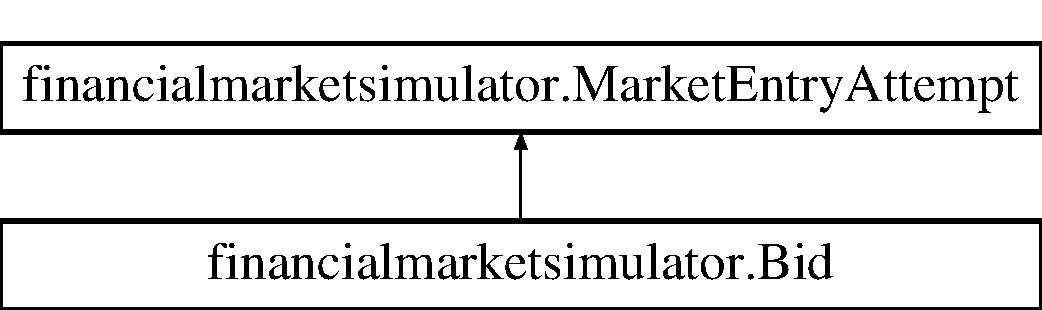
\includegraphics[height=2.000000cm]{classfinancialmarketsimulator_1_1_bid}
\end{center}
\end{figure}
\subsection*{Public Member Functions}
\begin{DoxyCompactItemize}
\item 
\hyperlink{classfinancialmarketsimulator_1_1_bid_a9ed8e389307df90419473a2b3ef375af}{Bid} ()
\item 
\hyperlink{classfinancialmarketsimulator_1_1_bid_a323008939bcfc7e51c56a9d61a1d79d9}{Bid} (double \+\_\+price, int \+\_\+num\+Shares, String \+\_\+name)
\end{DoxyCompactItemize}
\subsection*{Additional Inherited Members}


\subsection{Detailed Description}
\begin{DoxyAuthor}{Authors}
Madimetja Shika, Moeletji Semenya, Daniel Makgonta 
\end{DoxyAuthor}


Definition at line 9 of file Bid.\+java.



\subsection{Constructor \& Destructor Documentation}
\hypertarget{classfinancialmarketsimulator_1_1_bid_a9ed8e389307df90419473a2b3ef375af}{\index{financialmarketsimulator\+::\+Bid@{financialmarketsimulator\+::\+Bid}!Bid@{Bid}}
\index{Bid@{Bid}!financialmarketsimulator\+::\+Bid@{financialmarketsimulator\+::\+Bid}}
\subsubsection[{Bid}]{\setlength{\rightskip}{0pt plus 5cm}financialmarketsimulator.\+Bid.\+Bid (
\begin{DoxyParamCaption}
{}
\end{DoxyParamCaption}
)}}\label{classfinancialmarketsimulator_1_1_bid_a9ed8e389307df90419473a2b3ef375af}


Definition at line 11 of file Bid.\+java.

\hypertarget{classfinancialmarketsimulator_1_1_bid_a323008939bcfc7e51c56a9d61a1d79d9}{\index{financialmarketsimulator\+::\+Bid@{financialmarketsimulator\+::\+Bid}!Bid@{Bid}}
\index{Bid@{Bid}!financialmarketsimulator\+::\+Bid@{financialmarketsimulator\+::\+Bid}}
\subsubsection[{Bid}]{\setlength{\rightskip}{0pt plus 5cm}financialmarketsimulator.\+Bid.\+Bid (
\begin{DoxyParamCaption}
\item[{double}]{\+\_\+price, }
\item[{int}]{\+\_\+num\+Shares, }
\item[{String}]{\+\_\+name}
\end{DoxyParamCaption}
)}}\label{classfinancialmarketsimulator_1_1_bid_a323008939bcfc7e51c56a9d61a1d79d9}


Definition at line 16 of file Bid.\+java.



The documentation for this class was generated from the following file\+:\begin{DoxyCompactItemize}
\item 
C\+:/\+Users/\+Madimetja/\+Documents/\+Git\+Hub/bravo/\+Financial\+Market\+Simulator/src/financialmarketsimulator/\hyperlink{_bid_8java}{Bid.\+java}\end{DoxyCompactItemize}

\hypertarget{classfinancialmarketsimulator_1_1receipts_1_1_bid_receipt}{\section{financialmarketsimulator.\+receipts.\+Bid\+Receipt Class Reference}
\label{classfinancialmarketsimulator_1_1receipts_1_1_bid_receipt}\index{financialmarketsimulator.\+receipts.\+Bid\+Receipt@{financialmarketsimulator.\+receipts.\+Bid\+Receipt}}
}
Inheritance diagram for financialmarketsimulator.\+receipts.\+Bid\+Receipt\+:\begin{figure}[H]
\begin{center}
\leavevmode
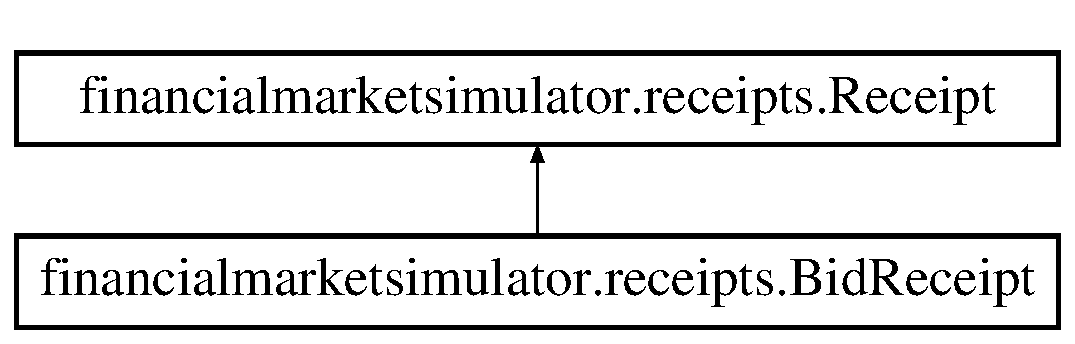
\includegraphics[height=2.000000cm]{classfinancialmarketsimulator_1_1receipts_1_1_bid_receipt}
\end{center}
\end{figure}


\subsection{Detailed Description}
\begin{DoxyAuthor}{Author}
Moeletji 
\end{DoxyAuthor}


Definition at line 13 of file Bid\+Receipt.\+java.



The documentation for this class was generated from the following file\+:\begin{DoxyCompactItemize}
\item 
C\+:/\+Users/\+Madimetja/\+Documents/\+Git\+Hub/bravo/\+Financial\+Market\+Simulator/src/financialmarketsimulator/receipts/Bid\+Receipt.\+java\end{DoxyCompactItemize}

\hypertarget{classfinancialmarketsimulator_1_1stack_1_1_bid_stack}{\section{financialmarketsimulator.\+stack.\+Bid\+Stack Class Reference}
\label{classfinancialmarketsimulator_1_1stack_1_1_bid_stack}\index{financialmarketsimulator.\+stack.\+Bid\+Stack@{financialmarketsimulator.\+stack.\+Bid\+Stack}}
}
Inheritance diagram for financialmarketsimulator.\+stack.\+Bid\+Stack\+:\begin{figure}[H]
\begin{center}
\leavevmode
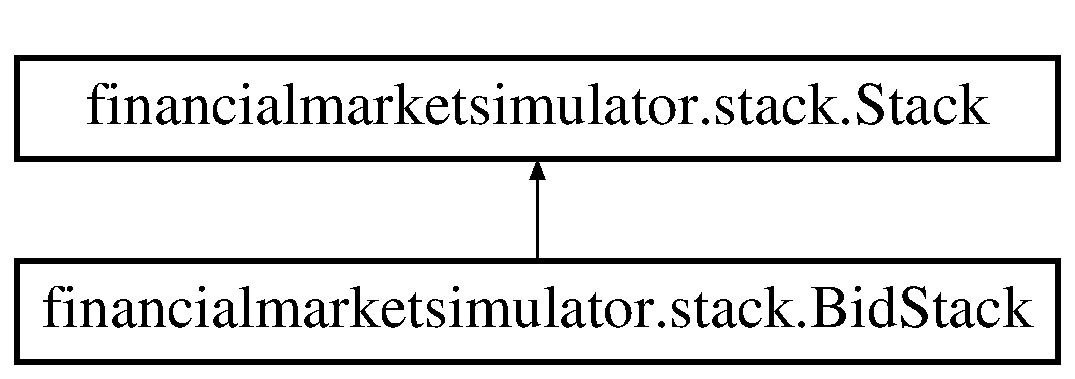
\includegraphics[height=2.000000cm]{classfinancialmarketsimulator_1_1stack_1_1_bid_stack}
\end{center}
\end{figure}
\subsection*{Public Member Functions}
\begin{DoxyCompactItemize}
\item 
void \hyperlink{classfinancialmarketsimulator_1_1stack_1_1_bid_stack_a5c2694a816c3fb93081f61554d60fc42}{sort\+Stack} ()
\end{DoxyCompactItemize}
\subsection*{Additional Inherited Members}


\subsection{Detailed Description}
\begin{DoxyAuthor}{Author}
Moeletji 
\end{DoxyAuthor}


Definition at line 13 of file Bid\+Stack.\+java.



\subsection{Member Function Documentation}
\hypertarget{classfinancialmarketsimulator_1_1stack_1_1_bid_stack_a5c2694a816c3fb93081f61554d60fc42}{\index{financialmarketsimulator\+::stack\+::\+Bid\+Stack@{financialmarketsimulator\+::stack\+::\+Bid\+Stack}!sort\+Stack@{sort\+Stack}}
\index{sort\+Stack@{sort\+Stack}!financialmarketsimulator\+::stack\+::\+Bid\+Stack@{financialmarketsimulator\+::stack\+::\+Bid\+Stack}}
\subsubsection[{sort\+Stack}]{\setlength{\rightskip}{0pt plus 5cm}void financialmarketsimulator.\+stack.\+Bid\+Stack.\+sort\+Stack (
\begin{DoxyParamCaption}
{}
\end{DoxyParamCaption}
)}}\label{classfinancialmarketsimulator_1_1stack_1_1_bid_stack_a5c2694a816c3fb93081f61554d60fc42}


Definition at line 15 of file Bid\+Stack.\+java.



The documentation for this class was generated from the following file\+:\begin{DoxyCompactItemize}
\item 
C\+:/\+Users/\+Madimetja/\+Documents/\+Git\+Hub/bravo/\+Financial\+Market\+Simulator/src/financialmarketsimulator/stack/\hyperlink{_bid_stack_8java}{Bid\+Stack.\+java}\end{DoxyCompactItemize}

\hypertarget{class_bid_unit_test}{\section{Bid\+Unit\+Test Class Reference}
\label{class_bid_unit_test}\index{Bid\+Unit\+Test@{Bid\+Unit\+Test}}
}
\subsection*{Public Member Functions}
\begin{DoxyCompactItemize}
\item 
\hypertarget{class_bid_unit_test_a17ac735be171e68824a4ab6aee2427c6}{void {\bfseries set\+Up} ()}\label{class_bid_unit_test_a17ac735be171e68824a4ab6aee2427c6}

\item 
\hypertarget{class_bid_unit_test_a1e3ac3daf16cfb03129bc9c6ec29004c}{void {\bfseries tear\+Down} ()}\label{class_bid_unit_test_a1e3ac3daf16cfb03129bc9c6ec29004c}

\item 
void \hyperlink{class_bid_unit_test_a00b30251528b2203d6d9f17c321bc499}{instantiation} ()
\end{DoxyCompactItemize}
\subsection*{Static Public Member Functions}
\begin{DoxyCompactItemize}
\item 
\hypertarget{class_bid_unit_test_a708398bb9f31d775f2a8cadfa7de00ad}{static void {\bfseries set\+Up\+Class} ()}\label{class_bid_unit_test_a708398bb9f31d775f2a8cadfa7de00ad}

\item 
\hypertarget{class_bid_unit_test_a63ef12d1e873a8b1dd37a8d1009a2a2f}{static void {\bfseries tear\+Down\+Class} ()}\label{class_bid_unit_test_a63ef12d1e873a8b1dd37a8d1009a2a2f}

\end{DoxyCompactItemize}


\subsection{Detailed Description}
\begin{DoxyAuthor}{Author}
Madimetja 
\end{DoxyAuthor}


Definition at line 18 of file Bid\+Unit\+Test.\+java.



\subsection{Member Function Documentation}
\hypertarget{class_bid_unit_test_a00b30251528b2203d6d9f17c321bc499}{\index{Bid\+Unit\+Test@{Bid\+Unit\+Test}!instantiation@{instantiation}}
\index{instantiation@{instantiation}!Bid\+Unit\+Test@{Bid\+Unit\+Test}}
\subsubsection[{instantiation}]{\setlength{\rightskip}{0pt plus 5cm}void Bid\+Unit\+Test.\+instantiation (
\begin{DoxyParamCaption}
{}
\end{DoxyParamCaption}
)}}\label{class_bid_unit_test_a00b30251528b2203d6d9f17c321bc499}
\begin{DoxyRefDesc}{Todo}
\item[\hyperlink{todo__todo000017}{Todo}]Tests if the Bid object instantiates as expected \end{DoxyRefDesc}


Definition at line 43 of file Bid\+Unit\+Test.\+java.



The documentation for this class was generated from the following file\+:\begin{DoxyCompactItemize}
\item 
C\+:/\+Users/\+Madimetja/\+Documents/\+Git\+Hub/bravo/\+Financial\+Market\+Simulator/test/Bid\+Unit\+Test.\+java\end{DoxyCompactItemize}

\hypertarget{classfinancialmarketsimulator_1_1exception_1_1_empty_exception}{\section{financialmarketsimulator.\+exception.\+Empty\+Exception Class Reference}
\label{classfinancialmarketsimulator_1_1exception_1_1_empty_exception}\index{financialmarketsimulator.\+exception.\+Empty\+Exception@{financialmarketsimulator.\+exception.\+Empty\+Exception}}
}
Inheritance diagram for financialmarketsimulator.\+exception.\+Empty\+Exception\+:\begin{figure}[H]
\begin{center}
\leavevmode
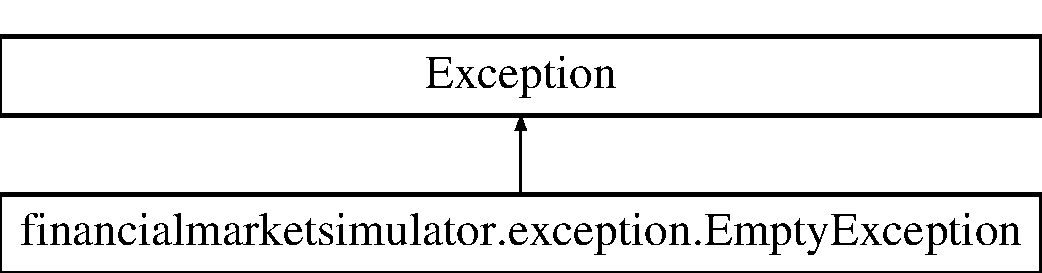
\includegraphics[height=2.000000cm]{classfinancialmarketsimulator_1_1exception_1_1_empty_exception}
\end{center}
\end{figure}


\subsection{Detailed Description}
\begin{DoxyAuthor}{Author}
Madimetja 
\end{DoxyAuthor}


Definition at line 12 of file Empty\+Exception.\+java.



The documentation for this class was generated from the following file\+:\begin{DoxyCompactItemize}
\item 
C\+:/\+Users/\+Madimetja/\+Documents/\+Git\+Hub/bravo/\+Financial\+Market\+Simulator/src/financialmarketsimulator/exception/Empty\+Exception.\+java\end{DoxyCompactItemize}

\hypertarget{class_exchange_unit_test}{\section{Exchange\+Unit\+Test Class Reference}
\label{class_exchange_unit_test}\index{Exchange\+Unit\+Test@{Exchange\+Unit\+Test}}
}
\subsection*{Public Member Functions}
\begin{DoxyCompactItemize}
\item 
\hypertarget{class_exchange_unit_test_a61dd0af902dc0da5513c53a2dc797b33}{void {\bfseries set\+Up} ()}\label{class_exchange_unit_test_a61dd0af902dc0da5513c53a2dc797b33}

\item 
\hypertarget{class_exchange_unit_test_a58164607cebb6763d2c7ab8866988cfb}{void {\bfseries tear\+Down} ()}\label{class_exchange_unit_test_a58164607cebb6763d2c7ab8866988cfb}

\item 
\hypertarget{class_exchange_unit_test_a7196c89003b25fcbe16ce03c95ad3cb6}{void {\bfseries instantiation} ()}\label{class_exchange_unit_test_a7196c89003b25fcbe16ce03c95ad3cb6}

\end{DoxyCompactItemize}
\subsection*{Static Public Member Functions}
\begin{DoxyCompactItemize}
\item 
\hypertarget{class_exchange_unit_test_abaa84464701e883f0938e6fdbe2b72b5}{static void {\bfseries set\+Up\+Class} ()}\label{class_exchange_unit_test_abaa84464701e883f0938e6fdbe2b72b5}

\item 
\hypertarget{class_exchange_unit_test_aeb8675a172645bd95fe665ad75f92bd5}{static void {\bfseries tear\+Down\+Class} ()}\label{class_exchange_unit_test_aeb8675a172645bd95fe665ad75f92bd5}

\end{DoxyCompactItemize}


\subsection{Detailed Description}
\begin{DoxyAuthor}{Author}
Madimetja 
\end{DoxyAuthor}


Definition at line 21 of file Exchange\+Unit\+Test.\+java.



The documentation for this class was generated from the following file\+:\begin{DoxyCompactItemize}
\item 
C\+:/\+Users/\+Madimetja/\+Documents/\+Git\+Hub/bravo/\+Financial\+Market\+Simulator/test/Exchange\+Unit\+Test.\+java\end{DoxyCompactItemize}

\hypertarget{classfinancialmarketsimulator_1_1_financial_market_simulator}{\section{financialmarketsimulator.\+Financial\+Market\+Simulator Class Reference}
\label{classfinancialmarketsimulator_1_1_financial_market_simulator}\index{financialmarketsimulator.\+Financial\+Market\+Simulator@{financialmarketsimulator.\+Financial\+Market\+Simulator}}
}
\subsection*{Static Public Member Functions}
\begin{DoxyCompactItemize}
\item 
static void \hyperlink{classfinancialmarketsimulator_1_1_financial_market_simulator_a55f0112537bdd6b3fb2607dd767d2ece}{main} (String\mbox{[}$\,$\mbox{]} args)
\end{DoxyCompactItemize}


\subsection{Detailed Description}
\begin{DoxyAuthor}{Authors}
Madimetja Shika, Moeletji Semenya, Daniel Makgonta 
\end{DoxyAuthor}


Definition at line 8 of file Financial\+Market\+Simulator.\+java.



\subsection{Member Function Documentation}
\hypertarget{classfinancialmarketsimulator_1_1_financial_market_simulator_a55f0112537bdd6b3fb2607dd767d2ece}{\index{financialmarketsimulator\+::\+Financial\+Market\+Simulator@{financialmarketsimulator\+::\+Financial\+Market\+Simulator}!main@{main}}
\index{main@{main}!financialmarketsimulator\+::\+Financial\+Market\+Simulator@{financialmarketsimulator\+::\+Financial\+Market\+Simulator}}
\subsubsection[{main}]{\setlength{\rightskip}{0pt plus 5cm}static void financialmarketsimulator.\+Financial\+Market\+Simulator.\+main (
\begin{DoxyParamCaption}
\item[{String\mbox{[}$\,$\mbox{]}}]{args}
\end{DoxyParamCaption}
)\hspace{0.3cm}{\ttfamily [static]}}}\label{classfinancialmarketsimulator_1_1_financial_market_simulator_a55f0112537bdd6b3fb2607dd767d2ece}


Definition at line 10 of file Financial\+Market\+Simulator.\+java.



The documentation for this class was generated from the following file\+:\begin{DoxyCompactItemize}
\item 
C\+:/\+Users/\+Madimetja/\+Documents/\+Git\+Hub/bravo/\+Financial\+Market\+Simulator/src/financialmarketsimulator/\hyperlink{_financial_market_simulator_8java}{Financial\+Market\+Simulator.\+java}\end{DoxyCompactItemize}

\hypertarget{classfinancialmarketsimulator_1_1exception_1_1_item_not_found_exception}{\section{financialmarketsimulator.\+exception.\+Item\+Not\+Found\+Exception Class Reference}
\label{classfinancialmarketsimulator_1_1exception_1_1_item_not_found_exception}\index{financialmarketsimulator.\+exception.\+Item\+Not\+Found\+Exception@{financialmarketsimulator.\+exception.\+Item\+Not\+Found\+Exception}}
}
Inheritance diagram for financialmarketsimulator.\+exception.\+Item\+Not\+Found\+Exception\+:\begin{figure}[H]
\begin{center}
\leavevmode
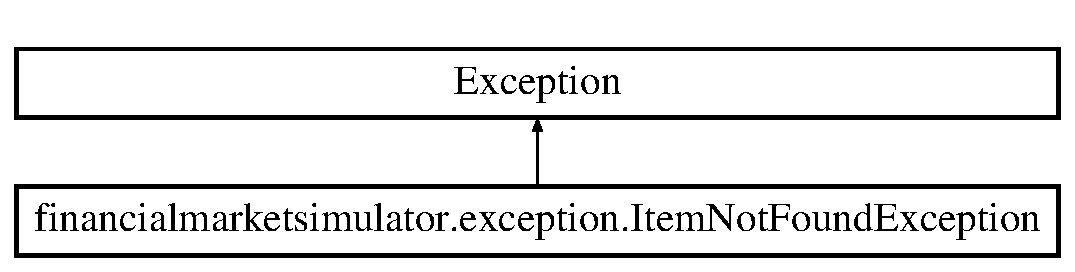
\includegraphics[height=2.000000cm]{classfinancialmarketsimulator_1_1exception_1_1_item_not_found_exception}
\end{center}
\end{figure}


\subsection{Detailed Description}
\begin{DoxyAuthor}{Authors}
Madimetja Shika, Moeletji Semenya, Daniel Makgonta 
\end{DoxyAuthor}


Definition at line 7 of file Item\+Not\+Found\+Exception.\+java.



The documentation for this class was generated from the following file\+:\begin{DoxyCompactItemize}
\item 
C\+:/\+Users/\+Madimetja/\+Documents/\+Git\+Hub/bravo/\+Financial\+Market\+Simulator/src/financialmarketsimulator/exception/Item\+Not\+Found\+Exception.\+java\end{DoxyCompactItemize}

\hypertarget{classfinancialmarketsimulator_1_1_market_entity}{\section{financialmarketsimulator.\+Market\+Entity Class Reference}
\label{classfinancialmarketsimulator_1_1_market_entity}\index{financialmarketsimulator.\+Market\+Entity@{financialmarketsimulator.\+Market\+Entity}}
}


\subsection{Detailed Description}
\begin{DoxyAuthor}{Authors}
Madimetja Shika, Moeletji Semenya, Daniel Makgonta 
\end{DoxyAuthor}


Definition at line 9 of file Market\+Entity.\+java.



The documentation for this class was generated from the following file\+:\begin{DoxyCompactItemize}
\item 
C\+:/\+Users/\+Madimetja/\+Documents/\+Git\+Hub/bravo/\+Financial\+Market\+Simulator/src/financialmarketsimulator/Market\+Entity.\+java\end{DoxyCompactItemize}

\hypertarget{class_market_entity_unit_test}{\section{Market\+Entity\+Unit\+Test Class Reference}
\label{class_market_entity_unit_test}\index{Market\+Entity\+Unit\+Test@{Market\+Entity\+Unit\+Test}}
}
\subsection*{Public Member Functions}
\begin{DoxyCompactItemize}
\item 
\hypertarget{class_market_entity_unit_test_a146492fa14011135db8b95abaeb1fe48}{void {\bfseries set\+Up} ()}\label{class_market_entity_unit_test_a146492fa14011135db8b95abaeb1fe48}

\item 
\hypertarget{class_market_entity_unit_test_abaa756813805984bc9dd42799d2712c4}{void {\bfseries tear\+Down} ()}\label{class_market_entity_unit_test_abaa756813805984bc9dd42799d2712c4}

\end{DoxyCompactItemize}
\subsection*{Static Public Member Functions}
\begin{DoxyCompactItemize}
\item 
\hypertarget{class_market_entity_unit_test_a55db93367ff6381d89024a48ab61b7e3}{static void {\bfseries set\+Up\+Class} ()}\label{class_market_entity_unit_test_a55db93367ff6381d89024a48ab61b7e3}

\item 
\hypertarget{class_market_entity_unit_test_a0fc27471ace003490b7088fd122a73a8}{static void {\bfseries tear\+Down\+Class} ()}\label{class_market_entity_unit_test_a0fc27471ace003490b7088fd122a73a8}

\end{DoxyCompactItemize}


\subsection{Detailed Description}
\begin{DoxyAuthor}{Author}
Madimetja 
\end{DoxyAuthor}


Definition at line 18 of file Market\+Entity\+Unit\+Test.\+java.



The documentation for this class was generated from the following file\+:\begin{DoxyCompactItemize}
\item 
C\+:/\+Users/\+Madimetja/\+Documents/\+Git\+Hub/bravo/\+Financial\+Market\+Simulator/test/Market\+Entity\+Unit\+Test.\+java\end{DoxyCompactItemize}

\hypertarget{classfinancialmarketsimulator_1_1_market_entry_attempt}{\section{financialmarketsimulator.\+Market\+Entry\+Attempt Class Reference}
\label{classfinancialmarketsimulator_1_1_market_entry_attempt}\index{financialmarketsimulator.\+Market\+Entry\+Attempt@{financialmarketsimulator.\+Market\+Entry\+Attempt}}
}
Inheritance diagram for financialmarketsimulator.\+Market\+Entry\+Attempt\+:\begin{figure}[H]
\begin{center}
\leavevmode
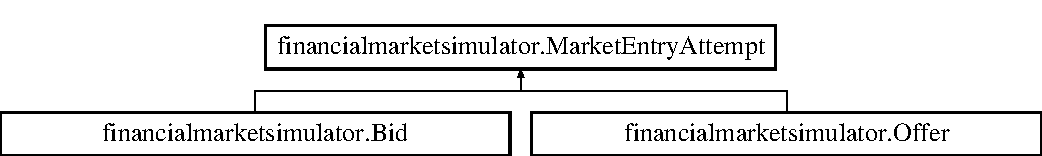
\includegraphics[height=2.000000cm]{classfinancialmarketsimulator_1_1_market_entry_attempt}
\end{center}
\end{figure}
\subsection*{Public Member Functions}
\begin{DoxyCompactItemize}
\item 
\hyperlink{classfinancialmarketsimulator_1_1_market_entry_attempt_a9b2f8a9eef7975bc053907e2ea05c779}{Market\+Entry\+Attempt} (double pr, int num\+Shares, String name)
\item 
double \hyperlink{classfinancialmarketsimulator_1_1_market_entry_attempt_a465bd475d2cf836c09e51e26ae937e66}{get\+Price} ()
\item 
int \hyperlink{classfinancialmarketsimulator_1_1_market_entry_attempt_ae48c6d1bc9ef23b88d077ee194686946}{get\+Number\+Of\+Shares} ()
\item 
String \hyperlink{classfinancialmarketsimulator_1_1_market_entry_attempt_a7c461ce88325da7ce771ef3e8284616c}{get\+Participant\+Name} ()
\item 
String \hyperlink{classfinancialmarketsimulator_1_1_market_entry_attempt_a48ec5ce3d7d0451da742f3290f0e3b52}{get\+Time\+Stanp} ()
\item 
void \hyperlink{classfinancialmarketsimulator_1_1_market_entry_attempt_ac350f88eed14da376cb58aa920df2f38}{set\+Price} (double \+\_\+price)
\item 
void \hyperlink{classfinancialmarketsimulator_1_1_market_entry_attempt_a27476573fd4a0aa03270c648500a3c98}{set\+Number\+Of\+Shares} (int \+\_\+num\+Shares)
\item 
void \hyperlink{classfinancialmarketsimulator_1_1_market_entry_attempt_af2b5d63e0ac8d2e39cf474e128739c8a}{set\+Participant\+Name} (String \+\_\+name)
\end{DoxyCompactItemize}
\subsection*{Protected Attributes}
\begin{DoxyCompactItemize}
\item 
double \hyperlink{classfinancialmarketsimulator_1_1_market_entry_attempt_a6e3074ceef1578108b239a355b0a6747}{price}
\item 
int \hyperlink{classfinancialmarketsimulator_1_1_market_entry_attempt_a5333f3fb0b26cba3382a05e582f86d8a}{number\+Of\+Shares}
\item 
String \hyperlink{classfinancialmarketsimulator_1_1_market_entry_attempt_a3b4418b6906b72597b72ec50a245afce}{participant\+Name}
\item 
Date \hyperlink{classfinancialmarketsimulator_1_1_market_entry_attempt_a7dcd3bab8cbe1498e452bec851e5ec5d}{date}
\item 
String \hyperlink{classfinancialmarketsimulator_1_1_market_entry_attempt_acd62492a481b9db42703ce1c60a01ff3}{time\+Stamp}
\end{DoxyCompactItemize}


\subsection{Detailed Description}
\begin{DoxyAuthor}{Author}
Madimetja 
\end{DoxyAuthor}


Definition at line 14 of file Market\+Entry\+Attempt.\+java.



\subsection{Constructor \& Destructor Documentation}
\hypertarget{classfinancialmarketsimulator_1_1_market_entry_attempt_a9b2f8a9eef7975bc053907e2ea05c779}{\index{financialmarketsimulator\+::\+Market\+Entry\+Attempt@{financialmarketsimulator\+::\+Market\+Entry\+Attempt}!Market\+Entry\+Attempt@{Market\+Entry\+Attempt}}
\index{Market\+Entry\+Attempt@{Market\+Entry\+Attempt}!financialmarketsimulator\+::\+Market\+Entry\+Attempt@{financialmarketsimulator\+::\+Market\+Entry\+Attempt}}
\subsubsection[{Market\+Entry\+Attempt}]{\setlength{\rightskip}{0pt plus 5cm}financialmarketsimulator.\+Market\+Entry\+Attempt.\+Market\+Entry\+Attempt (
\begin{DoxyParamCaption}
\item[{double}]{pr, }
\item[{int}]{num\+Shares, }
\item[{String}]{name}
\end{DoxyParamCaption}
)}}\label{classfinancialmarketsimulator_1_1_market_entry_attempt_a9b2f8a9eef7975bc053907e2ea05c779}
\begin{DoxyRefDesc}{Todo}
\item[\hyperlink{todo__todo000001}{Todo}]\hyperlink{classfinancialmarketsimulator_1_1_market_entry_attempt}{Market\+Entry\+Attempt} class constructor\end{DoxyRefDesc}



\begin{DoxyParams}{Parameters}
{\em pr} & The price of the entry attempt \\
\hline
{\em num\+Shares} & The number of shares being bid or offered \\
\hline
{\em name} & The name of the participant making the bid or the offer. \\
\hline
\end{DoxyParams}


Definition at line 51 of file Market\+Entry\+Attempt.\+java.



\subsection{Member Function Documentation}
\hypertarget{classfinancialmarketsimulator_1_1_market_entry_attempt_ae48c6d1bc9ef23b88d077ee194686946}{\index{financialmarketsimulator\+::\+Market\+Entry\+Attempt@{financialmarketsimulator\+::\+Market\+Entry\+Attempt}!get\+Number\+Of\+Shares@{get\+Number\+Of\+Shares}}
\index{get\+Number\+Of\+Shares@{get\+Number\+Of\+Shares}!financialmarketsimulator\+::\+Market\+Entry\+Attempt@{financialmarketsimulator\+::\+Market\+Entry\+Attempt}}
\subsubsection[{get\+Number\+Of\+Shares}]{\setlength{\rightskip}{0pt plus 5cm}int financialmarketsimulator.\+Market\+Entry\+Attempt.\+get\+Number\+Of\+Shares (
\begin{DoxyParamCaption}
{}
\end{DoxyParamCaption}
)}}\label{classfinancialmarketsimulator_1_1_market_entry_attempt_ae48c6d1bc9ef23b88d077ee194686946}
\begin{DoxyReturn}{Returns}
Integer value for the number of shares being offered or bid. 
\end{DoxyReturn}


Definition at line 69 of file Market\+Entry\+Attempt.\+java.

\hypertarget{classfinancialmarketsimulator_1_1_market_entry_attempt_a7c461ce88325da7ce771ef3e8284616c}{\index{financialmarketsimulator\+::\+Market\+Entry\+Attempt@{financialmarketsimulator\+::\+Market\+Entry\+Attempt}!get\+Participant\+Name@{get\+Participant\+Name}}
\index{get\+Participant\+Name@{get\+Participant\+Name}!financialmarketsimulator\+::\+Market\+Entry\+Attempt@{financialmarketsimulator\+::\+Market\+Entry\+Attempt}}
\subsubsection[{get\+Participant\+Name}]{\setlength{\rightskip}{0pt plus 5cm}String financialmarketsimulator.\+Market\+Entry\+Attempt.\+get\+Participant\+Name (
\begin{DoxyParamCaption}
{}
\end{DoxyParamCaption}
)}}\label{classfinancialmarketsimulator_1_1_market_entry_attempt_a7c461ce88325da7ce771ef3e8284616c}
\begin{DoxyReturn}{Returns}
String value for the name of the market participant who made the entry attempt. 
\end{DoxyReturn}


Definition at line 76 of file Market\+Entry\+Attempt.\+java.

\hypertarget{classfinancialmarketsimulator_1_1_market_entry_attempt_a465bd475d2cf836c09e51e26ae937e66}{\index{financialmarketsimulator\+::\+Market\+Entry\+Attempt@{financialmarketsimulator\+::\+Market\+Entry\+Attempt}!get\+Price@{get\+Price}}
\index{get\+Price@{get\+Price}!financialmarketsimulator\+::\+Market\+Entry\+Attempt@{financialmarketsimulator\+::\+Market\+Entry\+Attempt}}
\subsubsection[{get\+Price}]{\setlength{\rightskip}{0pt plus 5cm}double financialmarketsimulator.\+Market\+Entry\+Attempt.\+get\+Price (
\begin{DoxyParamCaption}
{}
\end{DoxyParamCaption}
)}}\label{classfinancialmarketsimulator_1_1_market_entry_attempt_a465bd475d2cf836c09e51e26ae937e66}
\begin{DoxyReturn}{Returns}
Double value for the price of the entry attempt, i.\+e. bid or offer 
\end{DoxyReturn}


Definition at line 62 of file Market\+Entry\+Attempt.\+java.

\hypertarget{classfinancialmarketsimulator_1_1_market_entry_attempt_a48ec5ce3d7d0451da742f3290f0e3b52}{\index{financialmarketsimulator\+::\+Market\+Entry\+Attempt@{financialmarketsimulator\+::\+Market\+Entry\+Attempt}!get\+Time\+Stanp@{get\+Time\+Stanp}}
\index{get\+Time\+Stanp@{get\+Time\+Stanp}!financialmarketsimulator\+::\+Market\+Entry\+Attempt@{financialmarketsimulator\+::\+Market\+Entry\+Attempt}}
\subsubsection[{get\+Time\+Stanp}]{\setlength{\rightskip}{0pt plus 5cm}String financialmarketsimulator.\+Market\+Entry\+Attempt.\+get\+Time\+Stanp (
\begin{DoxyParamCaption}
{}
\end{DoxyParamCaption}
)}}\label{classfinancialmarketsimulator_1_1_market_entry_attempt_a48ec5ce3d7d0451da742f3290f0e3b52}
\begin{DoxyReturn}{Returns}
String value representing time stamp of the entry attempt formatted as D\+D/\+M\+M/\+Y\+Y\+Y\+Y H\+H\+:\+M\+M\+:\+S\+S\+:M\+S T\+I\+M\+E\+\_\+\+Z\+O\+N\+E 
\end{DoxyReturn}


Definition at line 83 of file Market\+Entry\+Attempt.\+java.

\hypertarget{classfinancialmarketsimulator_1_1_market_entry_attempt_a27476573fd4a0aa03270c648500a3c98}{\index{financialmarketsimulator\+::\+Market\+Entry\+Attempt@{financialmarketsimulator\+::\+Market\+Entry\+Attempt}!set\+Number\+Of\+Shares@{set\+Number\+Of\+Shares}}
\index{set\+Number\+Of\+Shares@{set\+Number\+Of\+Shares}!financialmarketsimulator\+::\+Market\+Entry\+Attempt@{financialmarketsimulator\+::\+Market\+Entry\+Attempt}}
\subsubsection[{set\+Number\+Of\+Shares}]{\setlength{\rightskip}{0pt plus 5cm}void financialmarketsimulator.\+Market\+Entry\+Attempt.\+set\+Number\+Of\+Shares (
\begin{DoxyParamCaption}
\item[{int}]{\+\_\+num\+Shares}
\end{DoxyParamCaption}
)}}\label{classfinancialmarketsimulator_1_1_market_entry_attempt_a27476573fd4a0aa03270c648500a3c98}
\begin{DoxyRefDesc}{Todo}
\item[\hyperlink{todo__todo000003}{Todo}]Sets the number of shares for the entry attempt, i.\+e. the number of shares being offered or bid 
\begin{DoxyParams}{Parameters}
{\em \+\_\+num\+Shares} & The number of shares for the entry attempt. \\
\hline
\end{DoxyParams}
\end{DoxyRefDesc}


Definition at line 100 of file Market\+Entry\+Attempt.\+java.

\hypertarget{classfinancialmarketsimulator_1_1_market_entry_attempt_af2b5d63e0ac8d2e39cf474e128739c8a}{\index{financialmarketsimulator\+::\+Market\+Entry\+Attempt@{financialmarketsimulator\+::\+Market\+Entry\+Attempt}!set\+Participant\+Name@{set\+Participant\+Name}}
\index{set\+Participant\+Name@{set\+Participant\+Name}!financialmarketsimulator\+::\+Market\+Entry\+Attempt@{financialmarketsimulator\+::\+Market\+Entry\+Attempt}}
\subsubsection[{set\+Participant\+Name}]{\setlength{\rightskip}{0pt plus 5cm}void financialmarketsimulator.\+Market\+Entry\+Attempt.\+set\+Participant\+Name (
\begin{DoxyParamCaption}
\item[{String}]{\+\_\+name}
\end{DoxyParamCaption}
)}}\label{classfinancialmarketsimulator_1_1_market_entry_attempt_af2b5d63e0ac8d2e39cf474e128739c8a}
\begin{DoxyRefDesc}{Todo}
\item[\hyperlink{todo__todo000004}{Todo}]Sets the name of the participant making the entry attempt. 
\begin{DoxyParams}{Parameters}
{\em \+\_\+name} & The name of the participant making the entry attempt. \\
\hline
\end{DoxyParams}
\end{DoxyRefDesc}


Definition at line 109 of file Market\+Entry\+Attempt.\+java.

\hypertarget{classfinancialmarketsimulator_1_1_market_entry_attempt_ac350f88eed14da376cb58aa920df2f38}{\index{financialmarketsimulator\+::\+Market\+Entry\+Attempt@{financialmarketsimulator\+::\+Market\+Entry\+Attempt}!set\+Price@{set\+Price}}
\index{set\+Price@{set\+Price}!financialmarketsimulator\+::\+Market\+Entry\+Attempt@{financialmarketsimulator\+::\+Market\+Entry\+Attempt}}
\subsubsection[{set\+Price}]{\setlength{\rightskip}{0pt plus 5cm}void financialmarketsimulator.\+Market\+Entry\+Attempt.\+set\+Price (
\begin{DoxyParamCaption}
\item[{double}]{\+\_\+price}
\end{DoxyParamCaption}
)}}\label{classfinancialmarketsimulator_1_1_market_entry_attempt_ac350f88eed14da376cb58aa920df2f38}
\begin{DoxyRefDesc}{Todo}
\item[\hyperlink{todo__todo000002}{Todo}]Sets the price of the shares for entry attempt, i.\+e. sets the price of shares being offered or bid. 
\begin{DoxyParams}{Parameters}
{\em \+\_\+price} & The price of the shares for the entry attempt. \\
\hline
\end{DoxyParams}
\end{DoxyRefDesc}


Definition at line 91 of file Market\+Entry\+Attempt.\+java.



\subsection{Member Data Documentation}
\hypertarget{classfinancialmarketsimulator_1_1_market_entry_attempt_a7dcd3bab8cbe1498e452bec851e5ec5d}{\index{financialmarketsimulator\+::\+Market\+Entry\+Attempt@{financialmarketsimulator\+::\+Market\+Entry\+Attempt}!date@{date}}
\index{date@{date}!financialmarketsimulator\+::\+Market\+Entry\+Attempt@{financialmarketsimulator\+::\+Market\+Entry\+Attempt}}
\subsubsection[{date}]{\setlength{\rightskip}{0pt plus 5cm}Date financialmarketsimulator.\+Market\+Entry\+Attempt.\+date\hspace{0.3cm}{\ttfamily [protected]}}}\label{classfinancialmarketsimulator_1_1_market_entry_attempt_a7dcd3bab8cbe1498e452bec851e5ec5d}
Java Data variable to get current date. 

Definition at line 32 of file Market\+Entry\+Attempt.\+java.

\hypertarget{classfinancialmarketsimulator_1_1_market_entry_attempt_a5333f3fb0b26cba3382a05e582f86d8a}{\index{financialmarketsimulator\+::\+Market\+Entry\+Attempt@{financialmarketsimulator\+::\+Market\+Entry\+Attempt}!number\+Of\+Shares@{number\+Of\+Shares}}
\index{number\+Of\+Shares@{number\+Of\+Shares}!financialmarketsimulator\+::\+Market\+Entry\+Attempt@{financialmarketsimulator\+::\+Market\+Entry\+Attempt}}
\subsubsection[{number\+Of\+Shares}]{\setlength{\rightskip}{0pt plus 5cm}int financialmarketsimulator.\+Market\+Entry\+Attempt.\+number\+Of\+Shares\hspace{0.3cm}{\ttfamily [protected]}}}\label{classfinancialmarketsimulator_1_1_market_entry_attempt_a5333f3fb0b26cba3382a05e582f86d8a}
Stores the number of shares being offered of bid. 

Definition at line 24 of file Market\+Entry\+Attempt.\+java.

\hypertarget{classfinancialmarketsimulator_1_1_market_entry_attempt_a3b4418b6906b72597b72ec50a245afce}{\index{financialmarketsimulator\+::\+Market\+Entry\+Attempt@{financialmarketsimulator\+::\+Market\+Entry\+Attempt}!participant\+Name@{participant\+Name}}
\index{participant\+Name@{participant\+Name}!financialmarketsimulator\+::\+Market\+Entry\+Attempt@{financialmarketsimulator\+::\+Market\+Entry\+Attempt}}
\subsubsection[{participant\+Name}]{\setlength{\rightskip}{0pt plus 5cm}String financialmarketsimulator.\+Market\+Entry\+Attempt.\+participant\+Name\hspace{0.3cm}{\ttfamily [protected]}}}\label{classfinancialmarketsimulator_1_1_market_entry_attempt_a3b4418b6906b72597b72ec50a245afce}
Stores the name of the participant making the bid or offer. 

Definition at line 28 of file Market\+Entry\+Attempt.\+java.

\hypertarget{classfinancialmarketsimulator_1_1_market_entry_attempt_a6e3074ceef1578108b239a355b0a6747}{\index{financialmarketsimulator\+::\+Market\+Entry\+Attempt@{financialmarketsimulator\+::\+Market\+Entry\+Attempt}!price@{price}}
\index{price@{price}!financialmarketsimulator\+::\+Market\+Entry\+Attempt@{financialmarketsimulator\+::\+Market\+Entry\+Attempt}}
\subsubsection[{price}]{\setlength{\rightskip}{0pt plus 5cm}double financialmarketsimulator.\+Market\+Entry\+Attempt.\+price\hspace{0.3cm}{\ttfamily [protected]}}}\label{classfinancialmarketsimulator_1_1_market_entry_attempt_a6e3074ceef1578108b239a355b0a6747}
Stores the price of the entry attempt. This can be either a bid share price or an offer share price. 

Definition at line 20 of file Market\+Entry\+Attempt.\+java.

\hypertarget{classfinancialmarketsimulator_1_1_market_entry_attempt_acd62492a481b9db42703ce1c60a01ff3}{\index{financialmarketsimulator\+::\+Market\+Entry\+Attempt@{financialmarketsimulator\+::\+Market\+Entry\+Attempt}!time\+Stamp@{time\+Stamp}}
\index{time\+Stamp@{time\+Stamp}!financialmarketsimulator\+::\+Market\+Entry\+Attempt@{financialmarketsimulator\+::\+Market\+Entry\+Attempt}}
\subsubsection[{time\+Stamp}]{\setlength{\rightskip}{0pt plus 5cm}String financialmarketsimulator.\+Market\+Entry\+Attempt.\+time\+Stamp\hspace{0.3cm}{\ttfamily [protected]}}}\label{classfinancialmarketsimulator_1_1_market_entry_attempt_acd62492a481b9db42703ce1c60a01ff3}
Stores the date and time the offer or bid was made. 

Definition at line 36 of file Market\+Entry\+Attempt.\+java.



The documentation for this class was generated from the following file\+:\begin{DoxyCompactItemize}
\item 
C\+:/\+Users/\+Madimetja/\+Documents/\+Git\+Hub/bravo/\+Financial\+Market\+Simulator/src/financialmarketsimulator/Market\+Entry\+Attempt.\+java\end{DoxyCompactItemize}

\hypertarget{classfinancialmarketsimulator_1_1stack_1_1_market_entry_attempt_node}{\section{financialmarketsimulator.\+stack.\+Market\+Entry\+Attempt\+Node Class Reference}
\label{classfinancialmarketsimulator_1_1stack_1_1_market_entry_attempt_node}\index{financialmarketsimulator.\+stack.\+Market\+Entry\+Attempt\+Node@{financialmarketsimulator.\+stack.\+Market\+Entry\+Attempt\+Node}}
}
\subsection*{Public Member Functions}
\begin{DoxyCompactItemize}
\item 
\hyperlink{classfinancialmarketsimulator_1_1stack_1_1_market_entry_attempt_node_a1b07a62e05f0a51e7e77edbad7e1b07d}{Market\+Entry\+Attempt\+Node} (\hyperlink{classfinancialmarketsimulator_1_1_market_entry_attempt}{Market\+Entry\+Attempt} node1)
\end{DoxyCompactItemize}
\subsection*{Public Attributes}
\begin{DoxyCompactItemize}
\item 
\hyperlink{classfinancialmarketsimulator_1_1_market_entry_attempt}{Market\+Entry\+Attempt} \hyperlink{classfinancialmarketsimulator_1_1stack_1_1_market_entry_attempt_node_a9671342fa6e35efe9cbf03385e606f32}{next}
\item 
\hyperlink{classfinancialmarketsimulator_1_1_market_entry_attempt}{Market\+Entry\+Attempt} \hyperlink{classfinancialmarketsimulator_1_1stack_1_1_market_entry_attempt_node_a9a2784e51cab776b17f9957dbb2feb04}{node}
\end{DoxyCompactItemize}


\subsection{Detailed Description}
\begin{DoxyAuthor}{Author}
Madimetja 
\end{DoxyAuthor}


Definition at line 14 of file Market\+Entry\+Attempt\+Node.\+java.



\subsection{Constructor \& Destructor Documentation}
\hypertarget{classfinancialmarketsimulator_1_1stack_1_1_market_entry_attempt_node_a1b07a62e05f0a51e7e77edbad7e1b07d}{\index{financialmarketsimulator\+::stack\+::\+Market\+Entry\+Attempt\+Node@{financialmarketsimulator\+::stack\+::\+Market\+Entry\+Attempt\+Node}!Market\+Entry\+Attempt\+Node@{Market\+Entry\+Attempt\+Node}}
\index{Market\+Entry\+Attempt\+Node@{Market\+Entry\+Attempt\+Node}!financialmarketsimulator\+::stack\+::\+Market\+Entry\+Attempt\+Node@{financialmarketsimulator\+::stack\+::\+Market\+Entry\+Attempt\+Node}}
\subsubsection[{Market\+Entry\+Attempt\+Node}]{\setlength{\rightskip}{0pt plus 5cm}financialmarketsimulator.\+stack.\+Market\+Entry\+Attempt\+Node.\+Market\+Entry\+Attempt\+Node (
\begin{DoxyParamCaption}
\item[{{\bf Market\+Entry\+Attempt}}]{node1}
\end{DoxyParamCaption}
)}}\label{classfinancialmarketsimulator_1_1stack_1_1_market_entry_attempt_node_a1b07a62e05f0a51e7e77edbad7e1b07d}


Definition at line 19 of file Market\+Entry\+Attempt\+Node.\+java.



\subsection{Member Data Documentation}
\hypertarget{classfinancialmarketsimulator_1_1stack_1_1_market_entry_attempt_node_a9671342fa6e35efe9cbf03385e606f32}{\index{financialmarketsimulator\+::stack\+::\+Market\+Entry\+Attempt\+Node@{financialmarketsimulator\+::stack\+::\+Market\+Entry\+Attempt\+Node}!next@{next}}
\index{next@{next}!financialmarketsimulator\+::stack\+::\+Market\+Entry\+Attempt\+Node@{financialmarketsimulator\+::stack\+::\+Market\+Entry\+Attempt\+Node}}
\subsubsection[{next}]{\setlength{\rightskip}{0pt plus 5cm}{\bf Market\+Entry\+Attempt} financialmarketsimulator.\+stack.\+Market\+Entry\+Attempt\+Node.\+next}}\label{classfinancialmarketsimulator_1_1stack_1_1_market_entry_attempt_node_a9671342fa6e35efe9cbf03385e606f32}


Definition at line 16 of file Market\+Entry\+Attempt\+Node.\+java.

\hypertarget{classfinancialmarketsimulator_1_1stack_1_1_market_entry_attempt_node_a9a2784e51cab776b17f9957dbb2feb04}{\index{financialmarketsimulator\+::stack\+::\+Market\+Entry\+Attempt\+Node@{financialmarketsimulator\+::stack\+::\+Market\+Entry\+Attempt\+Node}!node@{node}}
\index{node@{node}!financialmarketsimulator\+::stack\+::\+Market\+Entry\+Attempt\+Node@{financialmarketsimulator\+::stack\+::\+Market\+Entry\+Attempt\+Node}}
\subsubsection[{node}]{\setlength{\rightskip}{0pt plus 5cm}{\bf Market\+Entry\+Attempt} financialmarketsimulator.\+stack.\+Market\+Entry\+Attempt\+Node.\+node}}\label{classfinancialmarketsimulator_1_1stack_1_1_market_entry_attempt_node_a9a2784e51cab776b17f9957dbb2feb04}


Definition at line 17 of file Market\+Entry\+Attempt\+Node.\+java.



The documentation for this class was generated from the following file\+:\begin{DoxyCompactItemize}
\item 
C\+:/\+Users/\+Madimetja/\+Documents/\+Git\+Hub/bravo/\+Financial\+Market\+Simulator/src/financialmarketsimulator/stack/\hyperlink{_market_entry_attempt_node_8java}{Market\+Entry\+Attempt\+Node.\+java}\end{DoxyCompactItemize}

\hypertarget{classstack_package_unit_tests_1_1_market_entry_attempt_node_unit_test}{\section{stack\+Package\+Unit\+Tests.\+Market\+Entry\+Attempt\+Node\+Unit\+Test Class Reference}
\label{classstack_package_unit_tests_1_1_market_entry_attempt_node_unit_test}\index{stack\+Package\+Unit\+Tests.\+Market\+Entry\+Attempt\+Node\+Unit\+Test@{stack\+Package\+Unit\+Tests.\+Market\+Entry\+Attempt\+Node\+Unit\+Test}}
}
\subsection*{Public Member Functions}
\begin{DoxyCompactItemize}
\item 
\hypertarget{classstack_package_unit_tests_1_1_market_entry_attempt_node_unit_test_a9390c1c0e025bf0b4e52d90e823b178e}{void {\bfseries set\+Up} ()}\label{classstack_package_unit_tests_1_1_market_entry_attempt_node_unit_test_a9390c1c0e025bf0b4e52d90e823b178e}

\item 
\hypertarget{classstack_package_unit_tests_1_1_market_entry_attempt_node_unit_test_ac53239c7d35e9cf1105772b0830bf111}{void {\bfseries tear\+Down} ()}\label{classstack_package_unit_tests_1_1_market_entry_attempt_node_unit_test_ac53239c7d35e9cf1105772b0830bf111}

\end{DoxyCompactItemize}
\subsection*{Static Public Member Functions}
\begin{DoxyCompactItemize}
\item 
\hypertarget{classstack_package_unit_tests_1_1_market_entry_attempt_node_unit_test_a4ca18c744d6e0e6ae6c71d18dc292e13}{static void {\bfseries set\+Up\+Class} ()}\label{classstack_package_unit_tests_1_1_market_entry_attempt_node_unit_test_a4ca18c744d6e0e6ae6c71d18dc292e13}

\item 
\hypertarget{classstack_package_unit_tests_1_1_market_entry_attempt_node_unit_test_af36feb95c6dbe4c59ce7f2014d7ba4ae}{static void {\bfseries tear\+Down\+Class} ()}\label{classstack_package_unit_tests_1_1_market_entry_attempt_node_unit_test_af36feb95c6dbe4c59ce7f2014d7ba4ae}

\end{DoxyCompactItemize}


\subsection{Detailed Description}
\begin{DoxyAuthor}{Author}
Madimetja 
\end{DoxyAuthor}


Definition at line 20 of file Market\+Entry\+Attempt\+Node\+Unit\+Test.\+java.



The documentation for this class was generated from the following file\+:\begin{DoxyCompactItemize}
\item 
C\+:/\+Users/\+Madimetja/\+Documents/\+Git\+Hub/bravo/\+Financial\+Market\+Simulator/test/stack\+Package\+Unit\+Tests/Market\+Entry\+Attempt\+Node\+Unit\+Test.\+java\end{DoxyCompactItemize}

\hypertarget{classfinancialmarketsimulator_1_1_market_manager}{\section{financialmarketsimulator.\+Market\+Manager Class Reference}
\label{classfinancialmarketsimulator_1_1_market_manager}\index{financialmarketsimulator.\+Market\+Manager@{financialmarketsimulator.\+Market\+Manager}}
}
\subsection*{Public Member Functions}
\begin{DoxyCompactItemize}
\item 
\hypertarget{classfinancialmarketsimulator_1_1_market_manager_abec3bfc62ba95bd12c444492b7cad61e}{{\bfseries Market\+Manager} (String s\+Name, String s\+Type, int num\+Shares, double val)}\label{classfinancialmarketsimulator_1_1_market_manager_abec3bfc62ba95bd12c444492b7cad61e}

\item 
\hypertarget{classfinancialmarketsimulator_1_1_market_manager_a468b11be3b1e2ce72f93dfc25468273b}{String {\bfseries accept\+Bid} (\hyperlink{classfinancialmarketsimulator_1_1_bid}{Bid} bid)}\label{classfinancialmarketsimulator_1_1_market_manager_a468b11be3b1e2ce72f93dfc25468273b}

\item 
\hypertarget{classfinancialmarketsimulator_1_1_market_manager_a2f9ad41c35ca0bb1ad2ac045f8cd3dd3}{String {\bfseries accept\+Offer} (\hyperlink{classfinancialmarketsimulator_1_1_offer}{Offer} offer)}\label{classfinancialmarketsimulator_1_1_market_manager_a2f9ad41c35ca0bb1ad2ac045f8cd3dd3}

\item 
\hypertarget{classfinancialmarketsimulator_1_1_market_manager_aa8c0454b1d66599ff5abbb01d35790e8}{String {\bfseries remove\+Bid} (\hyperlink{classfinancialmarketsimulator_1_1_bid}{Bid} bid)}\label{classfinancialmarketsimulator_1_1_market_manager_aa8c0454b1d66599ff5abbb01d35790e8}

\item 
\hypertarget{classfinancialmarketsimulator_1_1_market_manager_ad49a43c96b962562014c7bb37dfa5f7e}{String {\bfseries remove\+Offer} (\hyperlink{classfinancialmarketsimulator_1_1_offer}{Offer} offer)}\label{classfinancialmarketsimulator_1_1_market_manager_ad49a43c96b962562014c7bb37dfa5f7e}

\item 
\hypertarget{classfinancialmarketsimulator_1_1_market_manager_afb2bf557ed70cd23feccddfb5c01ab0d}{void {\bfseries update\+Engine} ()}\label{classfinancialmarketsimulator_1_1_market_manager_afb2bf557ed70cd23feccddfb5c01ab0d}

\item 
\hypertarget{classfinancialmarketsimulator_1_1_market_manager_a32d674b201543e3a6783ec64ba172266}{void {\bfseries update\+Entities} ()}\label{classfinancialmarketsimulator_1_1_market_manager_a32d674b201543e3a6783ec64ba172266}

\end{DoxyCompactItemize}


\subsection{Detailed Description}
\begin{DoxyAuthor}{Authors}
Madimetja Shika, Moeletji Semenya, Daniel Makgonta 
\end{DoxyAuthor}


Definition at line 10 of file Market\+Manager.\+java.



The documentation for this class was generated from the following file\+:\begin{DoxyCompactItemize}
\item 
C\+:/\+Users/\+Madimetja/\+Documents/\+Git\+Hub/bravo/\+Financial\+Market\+Simulator/src/financialmarketsimulator/Market\+Manager.\+java\end{DoxyCompactItemize}

\hypertarget{class_market_manager_unit_test}{\section{Market\+Manager\+Unit\+Test Class Reference}
\label{class_market_manager_unit_test}\index{Market\+Manager\+Unit\+Test@{Market\+Manager\+Unit\+Test}}
}
\subsection*{Public Member Functions}
\begin{DoxyCompactItemize}
\item 
\hypertarget{class_market_manager_unit_test_a7675c43ec3a21669742870c5ff7bcdef}{void {\bfseries set\+Up} ()}\label{class_market_manager_unit_test_a7675c43ec3a21669742870c5ff7bcdef}

\item 
\hypertarget{class_market_manager_unit_test_a8ce1dfb5c96973d49b3b1308bc9b77b9}{void {\bfseries tear\+Down} ()}\label{class_market_manager_unit_test_a8ce1dfb5c96973d49b3b1308bc9b77b9}

\item 
void \hyperlink{class_market_manager_unit_test_a975ffc40c27926b93d755a313440c35a}{instantiation} ()
\item 
void \hyperlink{class_market_manager_unit_test_aadbb351148ad8792ffdc73d21a477d46}{accept\+Bid\+Test} ()
\item 
void \hyperlink{class_market_manager_unit_test_a048bcd980b57e21cf535525c3d354327}{accept\+Offer\+Test} ()
\item 
void \hyperlink{class_market_manager_unit_test_ad15bca438fb420eb4edc10d2a6d5d69b}{remove\+Bid\+Test} ()
\item 
void \hyperlink{class_market_manager_unit_test_a3a39f91093490fa570428eeadbee53d8}{remove\+Offer\+Test} ()
\item 
void \hyperlink{class_market_manager_unit_test_a1c14446d8fae8ccdc8bbfb43054a5528}{update\+Engine\+Test} ()
\item 
void \hyperlink{class_market_manager_unit_test_ac830f868e90ae29122ae6382a4d227de}{update\+Entities\+Test} ()
\end{DoxyCompactItemize}
\subsection*{Static Public Member Functions}
\begin{DoxyCompactItemize}
\item 
\hypertarget{class_market_manager_unit_test_a5ecff1008c99832638bca96b9a12c129}{static void {\bfseries set\+Up\+Class} ()}\label{class_market_manager_unit_test_a5ecff1008c99832638bca96b9a12c129}

\item 
\hypertarget{class_market_manager_unit_test_a6384859a83037cf70ee3a30835e9067e}{static void {\bfseries tear\+Down\+Class} ()}\label{class_market_manager_unit_test_a6384859a83037cf70ee3a30835e9067e}

\end{DoxyCompactItemize}


\subsection{Detailed Description}
\begin{DoxyAuthor}{Author}
Madimetja 
\end{DoxyAuthor}


Definition at line 22 of file Market\+Manager\+Unit\+Test.\+java.



\subsection{Member Function Documentation}
\hypertarget{class_market_manager_unit_test_aadbb351148ad8792ffdc73d21a477d46}{\index{Market\+Manager\+Unit\+Test@{Market\+Manager\+Unit\+Test}!accept\+Bid\+Test@{accept\+Bid\+Test}}
\index{accept\+Bid\+Test@{accept\+Bid\+Test}!Market\+Manager\+Unit\+Test@{Market\+Manager\+Unit\+Test}}
\subsubsection[{accept\+Bid\+Test}]{\setlength{\rightskip}{0pt plus 5cm}void Market\+Manager\+Unit\+Test.\+accept\+Bid\+Test (
\begin{DoxyParamCaption}
{}
\end{DoxyParamCaption}
)}}\label{class_market_manager_unit_test_aadbb351148ad8792ffdc73d21a477d46}
\begin{DoxyRefDesc}{Todo}
\item[\hyperlink{todo__todo000018}{Todo}]\end{DoxyRefDesc}


Definition at line 63 of file Market\+Manager\+Unit\+Test.\+java.

\hypertarget{class_market_manager_unit_test_a048bcd980b57e21cf535525c3d354327}{\index{Market\+Manager\+Unit\+Test@{Market\+Manager\+Unit\+Test}!accept\+Offer\+Test@{accept\+Offer\+Test}}
\index{accept\+Offer\+Test@{accept\+Offer\+Test}!Market\+Manager\+Unit\+Test@{Market\+Manager\+Unit\+Test}}
\subsubsection[{accept\+Offer\+Test}]{\setlength{\rightskip}{0pt plus 5cm}void Market\+Manager\+Unit\+Test.\+accept\+Offer\+Test (
\begin{DoxyParamCaption}
{}
\end{DoxyParamCaption}
)}}\label{class_market_manager_unit_test_a048bcd980b57e21cf535525c3d354327}
\begin{DoxyRefDesc}{Todo}
\item[\hyperlink{todo__todo000019}{Todo}]\end{DoxyRefDesc}


Definition at line 74 of file Market\+Manager\+Unit\+Test.\+java.

\hypertarget{class_market_manager_unit_test_a975ffc40c27926b93d755a313440c35a}{\index{Market\+Manager\+Unit\+Test@{Market\+Manager\+Unit\+Test}!instantiation@{instantiation}}
\index{instantiation@{instantiation}!Market\+Manager\+Unit\+Test@{Market\+Manager\+Unit\+Test}}
\subsubsection[{instantiation}]{\setlength{\rightskip}{0pt plus 5cm}void Market\+Manager\+Unit\+Test.\+instantiation (
\begin{DoxyParamCaption}
{}
\end{DoxyParamCaption}
)}}\label{class_market_manager_unit_test_a975ffc40c27926b93d755a313440c35a}
Tests if the Market\+Manager object instantiates as expected 

Definition at line 52 of file Market\+Manager\+Unit\+Test.\+java.

\hypertarget{class_market_manager_unit_test_ad15bca438fb420eb4edc10d2a6d5d69b}{\index{Market\+Manager\+Unit\+Test@{Market\+Manager\+Unit\+Test}!remove\+Bid\+Test@{remove\+Bid\+Test}}
\index{remove\+Bid\+Test@{remove\+Bid\+Test}!Market\+Manager\+Unit\+Test@{Market\+Manager\+Unit\+Test}}
\subsubsection[{remove\+Bid\+Test}]{\setlength{\rightskip}{0pt plus 5cm}void Market\+Manager\+Unit\+Test.\+remove\+Bid\+Test (
\begin{DoxyParamCaption}
{}
\end{DoxyParamCaption}
)}}\label{class_market_manager_unit_test_ad15bca438fb420eb4edc10d2a6d5d69b}
\begin{DoxyRefDesc}{Todo}
\item[\hyperlink{todo__todo000020}{Todo}]\end{DoxyRefDesc}


Definition at line 85 of file Market\+Manager\+Unit\+Test.\+java.

\hypertarget{class_market_manager_unit_test_a3a39f91093490fa570428eeadbee53d8}{\index{Market\+Manager\+Unit\+Test@{Market\+Manager\+Unit\+Test}!remove\+Offer\+Test@{remove\+Offer\+Test}}
\index{remove\+Offer\+Test@{remove\+Offer\+Test}!Market\+Manager\+Unit\+Test@{Market\+Manager\+Unit\+Test}}
\subsubsection[{remove\+Offer\+Test}]{\setlength{\rightskip}{0pt plus 5cm}void Market\+Manager\+Unit\+Test.\+remove\+Offer\+Test (
\begin{DoxyParamCaption}
{}
\end{DoxyParamCaption}
)}}\label{class_market_manager_unit_test_a3a39f91093490fa570428eeadbee53d8}
\begin{DoxyRefDesc}{Todo}
\item[\hyperlink{todo__todo000021}{Todo}]\end{DoxyRefDesc}


Definition at line 96 of file Market\+Manager\+Unit\+Test.\+java.

\hypertarget{class_market_manager_unit_test_a1c14446d8fae8ccdc8bbfb43054a5528}{\index{Market\+Manager\+Unit\+Test@{Market\+Manager\+Unit\+Test}!update\+Engine\+Test@{update\+Engine\+Test}}
\index{update\+Engine\+Test@{update\+Engine\+Test}!Market\+Manager\+Unit\+Test@{Market\+Manager\+Unit\+Test}}
\subsubsection[{update\+Engine\+Test}]{\setlength{\rightskip}{0pt plus 5cm}void Market\+Manager\+Unit\+Test.\+update\+Engine\+Test (
\begin{DoxyParamCaption}
{}
\end{DoxyParamCaption}
)}}\label{class_market_manager_unit_test_a1c14446d8fae8ccdc8bbfb43054a5528}
\begin{DoxyRefDesc}{Todo}
\item[\hyperlink{todo__todo000022}{Todo}]\end{DoxyRefDesc}


Definition at line 107 of file Market\+Manager\+Unit\+Test.\+java.

\hypertarget{class_market_manager_unit_test_ac830f868e90ae29122ae6382a4d227de}{\index{Market\+Manager\+Unit\+Test@{Market\+Manager\+Unit\+Test}!update\+Entities\+Test@{update\+Entities\+Test}}
\index{update\+Entities\+Test@{update\+Entities\+Test}!Market\+Manager\+Unit\+Test@{Market\+Manager\+Unit\+Test}}
\subsubsection[{update\+Entities\+Test}]{\setlength{\rightskip}{0pt plus 5cm}void Market\+Manager\+Unit\+Test.\+update\+Entities\+Test (
\begin{DoxyParamCaption}
{}
\end{DoxyParamCaption}
)}}\label{class_market_manager_unit_test_ac830f868e90ae29122ae6382a4d227de}
\begin{DoxyRefDesc}{Todo}
\item[\hyperlink{todo__todo000023}{Todo}]\end{DoxyRefDesc}


Definition at line 115 of file Market\+Manager\+Unit\+Test.\+java.



The documentation for this class was generated from the following file\+:\begin{DoxyCompactItemize}
\item 
C\+:/\+Users/\+Madimetja/\+Documents/\+Git\+Hub/bravo/\+Financial\+Market\+Simulator/test/Market\+Manager\+Unit\+Test.\+java\end{DoxyCompactItemize}

\hypertarget{classfinancialmarketsimulator_1_1_market_strategy}{\section{financialmarketsimulator.\+Market\+Strategy Class Reference}
\label{classfinancialmarketsimulator_1_1_market_strategy}\index{financialmarketsimulator.\+Market\+Strategy@{financialmarketsimulator.\+Market\+Strategy}}
}
Inheritance diagram for financialmarketsimulator.\+Market\+Strategy\+:\begin{figure}[H]
\begin{center}
\leavevmode
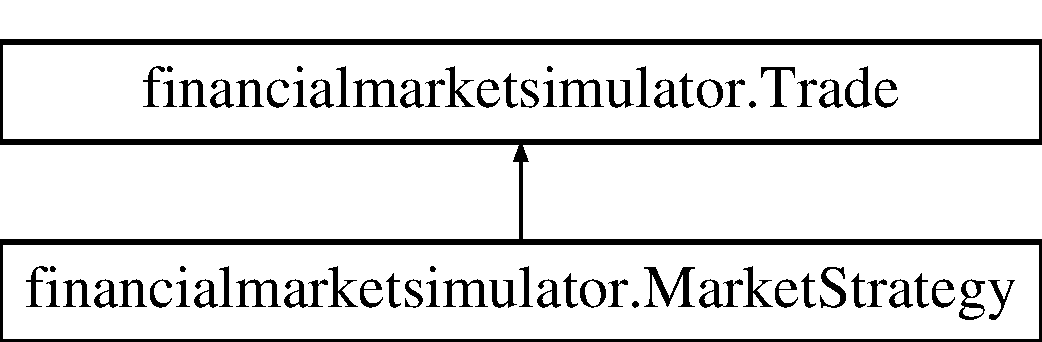
\includegraphics[height=2.000000cm]{classfinancialmarketsimulator_1_1_market_strategy}
\end{center}
\end{figure}
\subsection*{Public Member Functions}
\begin{DoxyCompactItemize}
\item 
\hypertarget{classfinancialmarketsimulator_1_1_market_strategy_a82e5b65bef66ffadea8085e3ca107130}{\hyperlink{classfinancialmarketsimulator_1_1_market_entry_attempt}{Market\+Entry\+Attempt} {\bfseries make\+Offer} ()}\label{classfinancialmarketsimulator_1_1_market_strategy_a82e5b65bef66ffadea8085e3ca107130}

\item 
\hypertarget{classfinancialmarketsimulator_1_1_market_strategy_a2a518f43a8460feab62ef5c31d0e02c9}{\hyperlink{classfinancialmarketsimulator_1_1_market_entry_attempt}{Market\+Entry\+Attempt} {\bfseries make\+Bid} ()}\label{classfinancialmarketsimulator_1_1_market_strategy_a2a518f43a8460feab62ef5c31d0e02c9}

\item 
\hypertarget{classfinancialmarketsimulator_1_1_market_strategy_ab7bbd10cab2e86f3c48c81bbb4c058e2}{void {\bfseries retract\+Bid} ()}\label{classfinancialmarketsimulator_1_1_market_strategy_ab7bbd10cab2e86f3c48c81bbb4c058e2}

\item 
\hypertarget{classfinancialmarketsimulator_1_1_market_strategy_aa3e0b344b5025ab9aa4a36df70b48ec3}{void {\bfseries retract\+Offer} ()}\label{classfinancialmarketsimulator_1_1_market_strategy_aa3e0b344b5025ab9aa4a36df70b48ec3}

\item 
\hypertarget{classfinancialmarketsimulator_1_1_market_strategy_ae65923e56266106ecb5b4b7f89a4e70b}{void {\bfseries set\+Strategy} (String strategy)}\label{classfinancialmarketsimulator_1_1_market_strategy_ae65923e56266106ecb5b4b7f89a4e70b}

\item 
\hypertarget{classfinancialmarketsimulator_1_1_market_strategy_ac773269f4e29a7b1099b3495d1781823}{\hyperlink{classfinancialmarketsimulator_1_1_market_entry_attempt}{Market\+Entry\+Attempt} {\bfseries search\+Market\+Entry\+Attempt} (\hyperlink{classfinancialmarketsimulator_1_1_market_entry_attempt}{Market\+Entry\+Attempt} entry)}\label{classfinancialmarketsimulator_1_1_market_strategy_ac773269f4e29a7b1099b3495d1781823}

\end{DoxyCompactItemize}


\subsection{Detailed Description}
\begin{DoxyAuthor}{Author}
Madimetja 
\end{DoxyAuthor}


Definition at line 12 of file Market\+Strategy.\+java.



The documentation for this class was generated from the following file\+:\begin{DoxyCompactItemize}
\item 
C\+:/\+Users/\+Madimetja/\+Documents/\+Git\+Hub/bravo/\+Financial\+Market\+Simulator/src/financialmarketsimulator/Market\+Strategy.\+java\end{DoxyCompactItemize}

\hypertarget{class_market_strategy_unit_test}{\section{Market\+Strategy\+Unit\+Test Class Reference}
\label{class_market_strategy_unit_test}\index{Market\+Strategy\+Unit\+Test@{Market\+Strategy\+Unit\+Test}}
}
\subsection*{Public Member Functions}
\begin{DoxyCompactItemize}
\item 
\hyperlink{class_market_strategy_unit_test_ae43ac2b179784a2176d37163c075fe7d}{Market\+Strategy\+Unit\+Test} ()
\item 
void \hyperlink{class_market_strategy_unit_test_aab34abed7a4e3829160450b21793da17}{set\+Up} ()
\item 
void \hyperlink{class_market_strategy_unit_test_afa4e0a0e8292236fbcf994dc042741fb}{tear\+Down} ()
\item 
void \hyperlink{class_market_strategy_unit_test_ab814f5c9983e0eaa02f7c5040b81971a}{make\+Offer\+Test} ()
\item 
void \hyperlink{class_market_strategy_unit_test_a98b0ebe10401ed5d3c9af160dfcb8f2a}{make\+Bid\+Test} ()
\item 
void \hyperlink{class_market_strategy_unit_test_aa0b0a03a9824cd06bc94c68d9c45042f}{retract\+Bid\+Test} ()
\item 
void \hyperlink{class_market_strategy_unit_test_a045225ba03abd2845f49e6c0e065712a}{retract\+Offer\+Test} ()
\item 
void \hyperlink{class_market_strategy_unit_test_ac701e483e622d7a918f1b8f21f024108}{set\+Strategy\+Test} ()
\item 
void \hyperlink{class_market_strategy_unit_test_a090ee23fae74dd8351ad91f17c784627}{search\+Market\+Entry\+Attempt} ()
\end{DoxyCompactItemize}
\subsection*{Static Public Member Functions}
\begin{DoxyCompactItemize}
\item 
static void \hyperlink{class_market_strategy_unit_test_ab6f9926edcaa9511516b0b3bb1025b9f}{set\+Up\+Class} ()
\item 
static void \hyperlink{class_market_strategy_unit_test_aeb485798bfb7f18a04b6355e6f2a2581}{tear\+Down\+Class} ()
\end{DoxyCompactItemize}


\subsection{Detailed Description}
\begin{DoxyAuthor}{Author}
Madimetja 
\end{DoxyAuthor}


Definition at line 18 of file Market\+Strategy\+Unit\+Test.\+java.



\subsection{Constructor \& Destructor Documentation}
\hypertarget{class_market_strategy_unit_test_ae43ac2b179784a2176d37163c075fe7d}{\index{Market\+Strategy\+Unit\+Test@{Market\+Strategy\+Unit\+Test}!Market\+Strategy\+Unit\+Test@{Market\+Strategy\+Unit\+Test}}
\index{Market\+Strategy\+Unit\+Test@{Market\+Strategy\+Unit\+Test}!Market\+Strategy\+Unit\+Test@{Market\+Strategy\+Unit\+Test}}
\subsubsection[{Market\+Strategy\+Unit\+Test}]{\setlength{\rightskip}{0pt plus 5cm}Market\+Strategy\+Unit\+Test.\+Market\+Strategy\+Unit\+Test (
\begin{DoxyParamCaption}
{}
\end{DoxyParamCaption}
)}}\label{class_market_strategy_unit_test_ae43ac2b179784a2176d37163c075fe7d}


Definition at line 20 of file Market\+Strategy\+Unit\+Test.\+java.



\subsection{Member Function Documentation}
\hypertarget{class_market_strategy_unit_test_a98b0ebe10401ed5d3c9af160dfcb8f2a}{\index{Market\+Strategy\+Unit\+Test@{Market\+Strategy\+Unit\+Test}!make\+Bid\+Test@{make\+Bid\+Test}}
\index{make\+Bid\+Test@{make\+Bid\+Test}!Market\+Strategy\+Unit\+Test@{Market\+Strategy\+Unit\+Test}}
\subsubsection[{make\+Bid\+Test}]{\setlength{\rightskip}{0pt plus 5cm}void Market\+Strategy\+Unit\+Test.\+make\+Bid\+Test (
\begin{DoxyParamCaption}
{}
\end{DoxyParamCaption}
)}}\label{class_market_strategy_unit_test_a98b0ebe10401ed5d3c9af160dfcb8f2a}
\begin{DoxyRefDesc}{Todo}
\item[\hyperlink{todo__todo000013}{Todo}]\end{DoxyRefDesc}


Definition at line 50 of file Market\+Strategy\+Unit\+Test.\+java.

\hypertarget{class_market_strategy_unit_test_ab814f5c9983e0eaa02f7c5040b81971a}{\index{Market\+Strategy\+Unit\+Test@{Market\+Strategy\+Unit\+Test}!make\+Offer\+Test@{make\+Offer\+Test}}
\index{make\+Offer\+Test@{make\+Offer\+Test}!Market\+Strategy\+Unit\+Test@{Market\+Strategy\+Unit\+Test}}
\subsubsection[{make\+Offer\+Test}]{\setlength{\rightskip}{0pt plus 5cm}void Market\+Strategy\+Unit\+Test.\+make\+Offer\+Test (
\begin{DoxyParamCaption}
{}
\end{DoxyParamCaption}
)}}\label{class_market_strategy_unit_test_ab814f5c9983e0eaa02f7c5040b81971a}
\begin{DoxyRefDesc}{Todo}
\item[\hyperlink{todo__todo000012}{Todo}]\end{DoxyRefDesc}


Definition at line 43 of file Market\+Strategy\+Unit\+Test.\+java.

\hypertarget{class_market_strategy_unit_test_aa0b0a03a9824cd06bc94c68d9c45042f}{\index{Market\+Strategy\+Unit\+Test@{Market\+Strategy\+Unit\+Test}!retract\+Bid\+Test@{retract\+Bid\+Test}}
\index{retract\+Bid\+Test@{retract\+Bid\+Test}!Market\+Strategy\+Unit\+Test@{Market\+Strategy\+Unit\+Test}}
\subsubsection[{retract\+Bid\+Test}]{\setlength{\rightskip}{0pt plus 5cm}void Market\+Strategy\+Unit\+Test.\+retract\+Bid\+Test (
\begin{DoxyParamCaption}
{}
\end{DoxyParamCaption}
)}}\label{class_market_strategy_unit_test_aa0b0a03a9824cd06bc94c68d9c45042f}
\begin{DoxyRefDesc}{Todo}
\item[\hyperlink{todo__todo000014}{Todo}]\end{DoxyRefDesc}


Definition at line 57 of file Market\+Strategy\+Unit\+Test.\+java.

\hypertarget{class_market_strategy_unit_test_a045225ba03abd2845f49e6c0e065712a}{\index{Market\+Strategy\+Unit\+Test@{Market\+Strategy\+Unit\+Test}!retract\+Offer\+Test@{retract\+Offer\+Test}}
\index{retract\+Offer\+Test@{retract\+Offer\+Test}!Market\+Strategy\+Unit\+Test@{Market\+Strategy\+Unit\+Test}}
\subsubsection[{retract\+Offer\+Test}]{\setlength{\rightskip}{0pt plus 5cm}void Market\+Strategy\+Unit\+Test.\+retract\+Offer\+Test (
\begin{DoxyParamCaption}
{}
\end{DoxyParamCaption}
)}}\label{class_market_strategy_unit_test_a045225ba03abd2845f49e6c0e065712a}
\begin{DoxyRefDesc}{Todo}
\item[\hyperlink{todo__todo000015}{Todo}]\end{DoxyRefDesc}


Definition at line 65 of file Market\+Strategy\+Unit\+Test.\+java.

\hypertarget{class_market_strategy_unit_test_a090ee23fae74dd8351ad91f17c784627}{\index{Market\+Strategy\+Unit\+Test@{Market\+Strategy\+Unit\+Test}!search\+Market\+Entry\+Attempt@{search\+Market\+Entry\+Attempt}}
\index{search\+Market\+Entry\+Attempt@{search\+Market\+Entry\+Attempt}!Market\+Strategy\+Unit\+Test@{Market\+Strategy\+Unit\+Test}}
\subsubsection[{search\+Market\+Entry\+Attempt}]{\setlength{\rightskip}{0pt plus 5cm}void Market\+Strategy\+Unit\+Test.\+search\+Market\+Entry\+Attempt (
\begin{DoxyParamCaption}
{}
\end{DoxyParamCaption}
)}}\label{class_market_strategy_unit_test_a090ee23fae74dd8351ad91f17c784627}
\begin{DoxyRefDesc}{Todo}
\item[\hyperlink{todo__todo000017}{Todo}]\end{DoxyRefDesc}


Definition at line 81 of file Market\+Strategy\+Unit\+Test.\+java.

\hypertarget{class_market_strategy_unit_test_ac701e483e622d7a918f1b8f21f024108}{\index{Market\+Strategy\+Unit\+Test@{Market\+Strategy\+Unit\+Test}!set\+Strategy\+Test@{set\+Strategy\+Test}}
\index{set\+Strategy\+Test@{set\+Strategy\+Test}!Market\+Strategy\+Unit\+Test@{Market\+Strategy\+Unit\+Test}}
\subsubsection[{set\+Strategy\+Test}]{\setlength{\rightskip}{0pt plus 5cm}void Market\+Strategy\+Unit\+Test.\+set\+Strategy\+Test (
\begin{DoxyParamCaption}
{}
\end{DoxyParamCaption}
)}}\label{class_market_strategy_unit_test_ac701e483e622d7a918f1b8f21f024108}
\begin{DoxyRefDesc}{Todo}
\item[\hyperlink{todo__todo000016}{Todo}]\end{DoxyRefDesc}


Definition at line 73 of file Market\+Strategy\+Unit\+Test.\+java.

\hypertarget{class_market_strategy_unit_test_aab34abed7a4e3829160450b21793da17}{\index{Market\+Strategy\+Unit\+Test@{Market\+Strategy\+Unit\+Test}!set\+Up@{set\+Up}}
\index{set\+Up@{set\+Up}!Market\+Strategy\+Unit\+Test@{Market\+Strategy\+Unit\+Test}}
\subsubsection[{set\+Up}]{\setlength{\rightskip}{0pt plus 5cm}void Market\+Strategy\+Unit\+Test.\+set\+Up (
\begin{DoxyParamCaption}
{}
\end{DoxyParamCaption}
)}}\label{class_market_strategy_unit_test_aab34abed7a4e3829160450b21793da17}


Definition at line 32 of file Market\+Strategy\+Unit\+Test.\+java.

\hypertarget{class_market_strategy_unit_test_ab6f9926edcaa9511516b0b3bb1025b9f}{\index{Market\+Strategy\+Unit\+Test@{Market\+Strategy\+Unit\+Test}!set\+Up\+Class@{set\+Up\+Class}}
\index{set\+Up\+Class@{set\+Up\+Class}!Market\+Strategy\+Unit\+Test@{Market\+Strategy\+Unit\+Test}}
\subsubsection[{set\+Up\+Class}]{\setlength{\rightskip}{0pt plus 5cm}static void Market\+Strategy\+Unit\+Test.\+set\+Up\+Class (
\begin{DoxyParamCaption}
{}
\end{DoxyParamCaption}
)\hspace{0.3cm}{\ttfamily [static]}}}\label{class_market_strategy_unit_test_ab6f9926edcaa9511516b0b3bb1025b9f}


Definition at line 24 of file Market\+Strategy\+Unit\+Test.\+java.

\hypertarget{class_market_strategy_unit_test_afa4e0a0e8292236fbcf994dc042741fb}{\index{Market\+Strategy\+Unit\+Test@{Market\+Strategy\+Unit\+Test}!tear\+Down@{tear\+Down}}
\index{tear\+Down@{tear\+Down}!Market\+Strategy\+Unit\+Test@{Market\+Strategy\+Unit\+Test}}
\subsubsection[{tear\+Down}]{\setlength{\rightskip}{0pt plus 5cm}void Market\+Strategy\+Unit\+Test.\+tear\+Down (
\begin{DoxyParamCaption}
{}
\end{DoxyParamCaption}
)}}\label{class_market_strategy_unit_test_afa4e0a0e8292236fbcf994dc042741fb}


Definition at line 36 of file Market\+Strategy\+Unit\+Test.\+java.

\hypertarget{class_market_strategy_unit_test_aeb485798bfb7f18a04b6355e6f2a2581}{\index{Market\+Strategy\+Unit\+Test@{Market\+Strategy\+Unit\+Test}!tear\+Down\+Class@{tear\+Down\+Class}}
\index{tear\+Down\+Class@{tear\+Down\+Class}!Market\+Strategy\+Unit\+Test@{Market\+Strategy\+Unit\+Test}}
\subsubsection[{tear\+Down\+Class}]{\setlength{\rightskip}{0pt plus 5cm}static void Market\+Strategy\+Unit\+Test.\+tear\+Down\+Class (
\begin{DoxyParamCaption}
{}
\end{DoxyParamCaption}
)\hspace{0.3cm}{\ttfamily [static]}}}\label{class_market_strategy_unit_test_aeb485798bfb7f18a04b6355e6f2a2581}


Definition at line 28 of file Market\+Strategy\+Unit\+Test.\+java.



The documentation for this class was generated from the following file\+:\begin{DoxyCompactItemize}
\item 
C\+:/\+Users/\+Madimetja/\+Documents/\+Git\+Hub/bravo/\+Financial\+Market\+Simulator/test/\hyperlink{_market_strategy_unit_test_8java}{Market\+Strategy\+Unit\+Test.\+java}\end{DoxyCompactItemize}

\hypertarget{classfinancialmarketsimulator_1_1_matching_engine}{\section{financialmarketsimulator.\+Matching\+Engine Class Reference}
\label{classfinancialmarketsimulator_1_1_matching_engine}\index{financialmarketsimulator.\+Matching\+Engine@{financialmarketsimulator.\+Matching\+Engine}}
}
\subsection*{Public Member Functions}
\begin{DoxyCompactItemize}
\item 
\hyperlink{classfinancialmarketsimulator_1_1_matching_engine_a2b6448ca83b5c11a9e48afd1286a6bb0}{Matching\+Engine} ()
\item 
void \hyperlink{classfinancialmarketsimulator_1_1_matching_engine_aa835268cf4fa1feff9f528b72cadd57f}{trade} ()
\item 
void \hyperlink{classfinancialmarketsimulator_1_1_matching_engine_a7a5e112f743728b6ea9d62d263fb74e3}{update} ()
\end{DoxyCompactItemize}


\subsection{Detailed Description}
\begin{DoxyAuthor}{Authors}
Madimetja Shika, Moeletji Semenya, Daniel Makgonta 
\end{DoxyAuthor}


Definition at line 7 of file Matching\+Engine.\+java.



\subsection{Constructor \& Destructor Documentation}
\hypertarget{classfinancialmarketsimulator_1_1_matching_engine_a2b6448ca83b5c11a9e48afd1286a6bb0}{\index{financialmarketsimulator\+::\+Matching\+Engine@{financialmarketsimulator\+::\+Matching\+Engine}!Matching\+Engine@{Matching\+Engine}}
\index{Matching\+Engine@{Matching\+Engine}!financialmarketsimulator\+::\+Matching\+Engine@{financialmarketsimulator\+::\+Matching\+Engine}}
\subsubsection[{Matching\+Engine}]{\setlength{\rightskip}{0pt plus 5cm}financialmarketsimulator.\+Matching\+Engine.\+Matching\+Engine (
\begin{DoxyParamCaption}
{}
\end{DoxyParamCaption}
)}}\label{classfinancialmarketsimulator_1_1_matching_engine_a2b6448ca83b5c11a9e48afd1286a6bb0}


Definition at line 9 of file Matching\+Engine.\+java.



\subsection{Member Function Documentation}
\hypertarget{classfinancialmarketsimulator_1_1_matching_engine_aa835268cf4fa1feff9f528b72cadd57f}{\index{financialmarketsimulator\+::\+Matching\+Engine@{financialmarketsimulator\+::\+Matching\+Engine}!trade@{trade}}
\index{trade@{trade}!financialmarketsimulator\+::\+Matching\+Engine@{financialmarketsimulator\+::\+Matching\+Engine}}
\subsubsection[{trade}]{\setlength{\rightskip}{0pt plus 5cm}void financialmarketsimulator.\+Matching\+Engine.\+trade (
\begin{DoxyParamCaption}
{}
\end{DoxyParamCaption}
)}}\label{classfinancialmarketsimulator_1_1_matching_engine_aa835268cf4fa1feff9f528b72cadd57f}


Definition at line 14 of file Matching\+Engine.\+java.

\hypertarget{classfinancialmarketsimulator_1_1_matching_engine_a7a5e112f743728b6ea9d62d263fb74e3}{\index{financialmarketsimulator\+::\+Matching\+Engine@{financialmarketsimulator\+::\+Matching\+Engine}!update@{update}}
\index{update@{update}!financialmarketsimulator\+::\+Matching\+Engine@{financialmarketsimulator\+::\+Matching\+Engine}}
\subsubsection[{update}]{\setlength{\rightskip}{0pt plus 5cm}void financialmarketsimulator.\+Matching\+Engine.\+update (
\begin{DoxyParamCaption}
{}
\end{DoxyParamCaption}
)}}\label{classfinancialmarketsimulator_1_1_matching_engine_a7a5e112f743728b6ea9d62d263fb74e3}


Definition at line 19 of file Matching\+Engine.\+java.



The documentation for this class was generated from the following file\+:\begin{DoxyCompactItemize}
\item 
C\+:/\+Users/\+Madimetja/\+Documents/\+Git\+Hub/bravo/\+Financial\+Market\+Simulator/src/financialmarketsimulator/\hyperlink{_matching_engine_8java}{Matching\+Engine.\+java}\end{DoxyCompactItemize}

\hypertarget{class_matching_engine_unit_test}{\section{Matching\+Engine\+Unit\+Test Class Reference}
\label{class_matching_engine_unit_test}\index{Matching\+Engine\+Unit\+Test@{Matching\+Engine\+Unit\+Test}}
}
\subsection*{Public Member Functions}
\begin{DoxyCompactItemize}
\item 
\hypertarget{class_matching_engine_unit_test_a2fe9413d67e2ad0c8233d11d1f209548}{void {\bfseries set\+Up} ()}\label{class_matching_engine_unit_test_a2fe9413d67e2ad0c8233d11d1f209548}

\item 
\hypertarget{class_matching_engine_unit_test_adececd49e895e978d85a27b8470104d3}{void {\bfseries tear\+Down} ()}\label{class_matching_engine_unit_test_adececd49e895e978d85a27b8470104d3}

\item 
\hypertarget{class_matching_engine_unit_test_acbb8d543a15e349d8f46769388fd28bd}{void {\bfseries instantiation} ()}\label{class_matching_engine_unit_test_acbb8d543a15e349d8f46769388fd28bd}

\item 
\hypertarget{class_matching_engine_unit_test_a2dbbdf5632bac8d35d6902caf5556c5f}{void {\bfseries trade\+Test} ()}\label{class_matching_engine_unit_test_a2dbbdf5632bac8d35d6902caf5556c5f}

\item 
\hypertarget{class_matching_engine_unit_test_a914f15f54087d84798e02b33734a9791}{void {\bfseries update\+Test} ()}\label{class_matching_engine_unit_test_a914f15f54087d84798e02b33734a9791}

\end{DoxyCompactItemize}
\subsection*{Static Public Member Functions}
\begin{DoxyCompactItemize}
\item 
\hypertarget{class_matching_engine_unit_test_a35f673f5cdf8f8282686a1f84ee2dd37}{static void {\bfseries set\+Up\+Class} ()}\label{class_matching_engine_unit_test_a35f673f5cdf8f8282686a1f84ee2dd37}

\item 
\hypertarget{class_matching_engine_unit_test_a0fb23de300ffd3a7d2b42e84d457be09}{static void {\bfseries tear\+Down\+Class} ()}\label{class_matching_engine_unit_test_a0fb23de300ffd3a7d2b42e84d457be09}

\end{DoxyCompactItemize}


\subsection{Detailed Description}
\begin{DoxyAuthor}{Author}
Madimetja 
\end{DoxyAuthor}


Definition at line 23 of file Matching\+Engine\+Unit\+Test.\+java.



The documentation for this class was generated from the following file\+:\begin{DoxyCompactItemize}
\item 
C\+:/\+Users/\+Madimetja/\+Documents/\+Git\+Hub/bravo/\+Financial\+Market\+Simulator/test/Matching\+Engine\+Unit\+Test.\+java\end{DoxyCompactItemize}

\hypertarget{classfinancialmarketsimulator_1_1_offer}{\section{financialmarketsimulator.\+Offer Class Reference}
\label{classfinancialmarketsimulator_1_1_offer}\index{financialmarketsimulator.\+Offer@{financialmarketsimulator.\+Offer}}
}
Inheritance diagram for financialmarketsimulator.\+Offer\+:\begin{figure}[H]
\begin{center}
\leavevmode
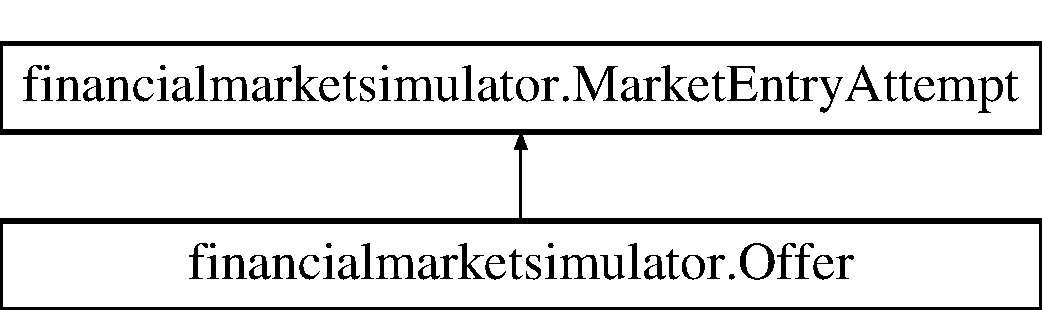
\includegraphics[height=2.000000cm]{classfinancialmarketsimulator_1_1_offer}
\end{center}
\end{figure}
\subsection*{Public Member Functions}
\begin{DoxyCompactItemize}
\item 
\hypertarget{classfinancialmarketsimulator_1_1_offer_a155651fa401d386b3e97067f02300b18}{{\bfseries Offer} (double \+\_\+price, int \+\_\+num\+Shares, String \+\_\+name)}\label{classfinancialmarketsimulator_1_1_offer_a155651fa401d386b3e97067f02300b18}

\end{DoxyCompactItemize}
\subsection*{Additional Inherited Members}


\subsection{Detailed Description}
\begin{DoxyAuthor}{Authors}
Madimetja Shika, Moeletji Semenya, Daniel Makgonta 
\end{DoxyAuthor}


Definition at line 9 of file Offer.\+java.



The documentation for this class was generated from the following file\+:\begin{DoxyCompactItemize}
\item 
C\+:/\+Users/\+Madimetja/\+Documents/\+Git\+Hub/bravo/\+Financial\+Market\+Simulator/src/financialmarketsimulator/Offer.\+java\end{DoxyCompactItemize}

\hypertarget{classfinancialmarketsimulator_1_1receipts_1_1_offer_receipt}{\section{financialmarketsimulator.\+receipts.\+Offer\+Receipt Class Reference}
\label{classfinancialmarketsimulator_1_1receipts_1_1_offer_receipt}\index{financialmarketsimulator.\+receipts.\+Offer\+Receipt@{financialmarketsimulator.\+receipts.\+Offer\+Receipt}}
}


\subsection{Detailed Description}
\begin{DoxyAuthor}{Author}
Moeletji 
\end{DoxyAuthor}


Definition at line 13 of file Offer\+Receipt.\+java.



The documentation for this class was generated from the following file\+:\begin{DoxyCompactItemize}
\item 
C\+:/\+Users/\+Madimetja/\+Documents/\+Git\+Hub/bravo/\+Financial\+Market\+Simulator/src/financialmarketsimulator/receipts/\hyperlink{_offer_receipt_8java}{Offer\+Receipt.\+java}\end{DoxyCompactItemize}

\hypertarget{classfinancialmarketsimulator_1_1stack_1_1_offer_stack}{\section{financialmarketsimulator.\+stack.\+Offer\+Stack Class Reference}
\label{classfinancialmarketsimulator_1_1stack_1_1_offer_stack}\index{financialmarketsimulator.\+stack.\+Offer\+Stack@{financialmarketsimulator.\+stack.\+Offer\+Stack}}
}
Inheritance diagram for financialmarketsimulator.\+stack.\+Offer\+Stack\+:\begin{figure}[H]
\begin{center}
\leavevmode
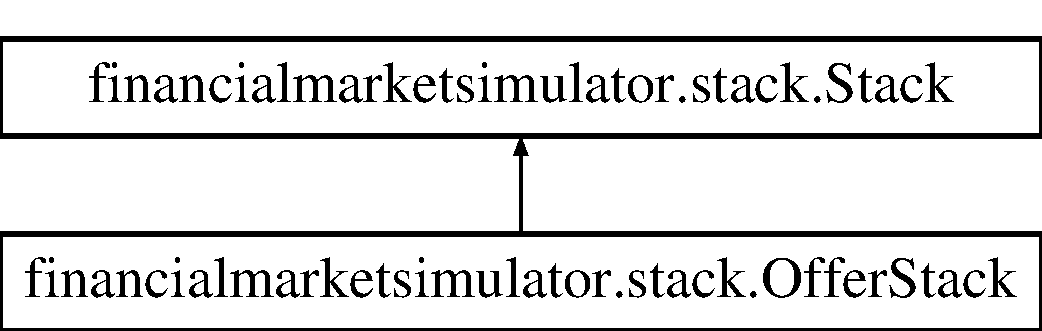
\includegraphics[height=2.000000cm]{classfinancialmarketsimulator_1_1stack_1_1_offer_stack}
\end{center}
\end{figure}
\subsection*{Public Member Functions}
\begin{DoxyCompactItemize}
\item 
\hypertarget{classfinancialmarketsimulator_1_1stack_1_1_offer_stack_a34bc18d02e364310b528b9a40f58d16f}{void {\bfseries sort\+Stack} ()}\label{classfinancialmarketsimulator_1_1stack_1_1_offer_stack_a34bc18d02e364310b528b9a40f58d16f}

\end{DoxyCompactItemize}
\subsection*{Additional Inherited Members}


\subsection{Detailed Description}
\begin{DoxyAuthor}{Author}
Moeletji 
\end{DoxyAuthor}


Definition at line 13 of file Offer\+Stack.\+java.



The documentation for this class was generated from the following file\+:\begin{DoxyCompactItemize}
\item 
C\+:/\+Users/\+Madimetja/\+Documents/\+Git\+Hub/bravo/\+Financial\+Market\+Simulator/src/financialmarketsimulator/stack/Offer\+Stack.\+java\end{DoxyCompactItemize}

\hypertarget{class_offer_unit_test}{\section{Offer\+Unit\+Test Class Reference}
\label{class_offer_unit_test}\index{Offer\+Unit\+Test@{Offer\+Unit\+Test}}
}
\subsection*{Public Member Functions}
\begin{DoxyCompactItemize}
\item 
\hypertarget{class_offer_unit_test_a491087ff4d8fd6bad517f3e65c6a2c1a}{void {\bfseries set\+Up} ()}\label{class_offer_unit_test_a491087ff4d8fd6bad517f3e65c6a2c1a}

\item 
\hypertarget{class_offer_unit_test_a8e3f348a59b90790bb602bafbe7e2c0d}{void {\bfseries tear\+Down} ()}\label{class_offer_unit_test_a8e3f348a59b90790bb602bafbe7e2c0d}

\item 
\hypertarget{class_offer_unit_test_a6a183dfb778383f20231c0dd4a43dc65}{void {\bfseries instantiation} ()}\label{class_offer_unit_test_a6a183dfb778383f20231c0dd4a43dc65}

\end{DoxyCompactItemize}
\subsection*{Static Public Member Functions}
\begin{DoxyCompactItemize}
\item 
\hypertarget{class_offer_unit_test_a814f87470fbd7747577a8d21a1e31374}{static void {\bfseries set\+Up\+Class} ()}\label{class_offer_unit_test_a814f87470fbd7747577a8d21a1e31374}

\item 
\hypertarget{class_offer_unit_test_afcf0203b47fec4b0899c2e53f2a1a4dc}{static void {\bfseries tear\+Down\+Class} ()}\label{class_offer_unit_test_afcf0203b47fec4b0899c2e53f2a1a4dc}

\end{DoxyCompactItemize}


\subsection{Detailed Description}
\begin{DoxyAuthor}{Author}
Madimetja 
\end{DoxyAuthor}


Definition at line 18 of file Offer\+Unit\+Test.\+java.



The documentation for this class was generated from the following file\+:\begin{DoxyCompactItemize}
\item 
C\+:/\+Users/\+Madimetja/\+Documents/\+Git\+Hub/bravo/\+Financial\+Market\+Simulator/test/Offer\+Unit\+Test.\+java\end{DoxyCompactItemize}

\hypertarget{classfinancialmarketsimulator_1_1receipts_1_1_receipt}{\section{financialmarketsimulator.\+receipts.\+Receipt Class Reference}
\label{classfinancialmarketsimulator_1_1receipts_1_1_receipt}\index{financialmarketsimulator.\+receipts.\+Receipt@{financialmarketsimulator.\+receipts.\+Receipt}}
}
Inheritance diagram for financialmarketsimulator.\+receipts.\+Receipt\+:\begin{figure}[H]
\begin{center}
\leavevmode
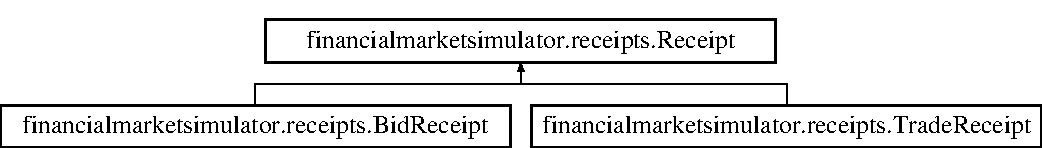
\includegraphics[height=1.978799cm]{classfinancialmarketsimulator_1_1receipts_1_1_receipt}
\end{center}
\end{figure}


\subsection{Detailed Description}
\begin{DoxyAuthor}{Author}
Moeletji 
\end{DoxyAuthor}


Definition at line 13 of file Receipt.\+java.



The documentation for this class was generated from the following file\+:\begin{DoxyCompactItemize}
\item 
C\+:/\+Users/\+Madimetja/\+Documents/\+Git\+Hub/bravo/\+Financial\+Market\+Simulator/src/financialmarketsimulator/receipts/Receipt.\+java\end{DoxyCompactItemize}

\hypertarget{class_receipt_unit_test}{\section{Receipt\+Unit\+Test Class Reference}
\label{class_receipt_unit_test}\index{Receipt\+Unit\+Test@{Receipt\+Unit\+Test}}
}
\subsection*{Public Member Functions}
\begin{DoxyCompactItemize}
\item 
\hypertarget{class_receipt_unit_test_aac78b41793c52301090b041a76a7990d}{void {\bfseries set\+Up} ()}\label{class_receipt_unit_test_aac78b41793c52301090b041a76a7990d}

\item 
\hypertarget{class_receipt_unit_test_af07963be2cea104cb428a55a6216fc68}{void {\bfseries tear\+Down} ()}\label{class_receipt_unit_test_af07963be2cea104cb428a55a6216fc68}

\item 
void \hyperlink{class_receipt_unit_test_aab92fcc0a866db8ec56ed65b9693cdc8}{instantiation} ()
\end{DoxyCompactItemize}
\subsection*{Static Public Member Functions}
\begin{DoxyCompactItemize}
\item 
\hypertarget{class_receipt_unit_test_a349b50a6df17f5b573210fab7cb7ed50}{static void {\bfseries set\+Up\+Class} ()}\label{class_receipt_unit_test_a349b50a6df17f5b573210fab7cb7ed50}

\item 
\hypertarget{class_receipt_unit_test_a16caf64de74462999a3e508979cb4438}{static void {\bfseries tear\+Down\+Class} ()}\label{class_receipt_unit_test_a16caf64de74462999a3e508979cb4438}

\end{DoxyCompactItemize}


\subsection{Detailed Description}
\begin{DoxyAuthor}{Author}
Madimetja 
\end{DoxyAuthor}


Definition at line 18 of file Receipt\+Unit\+Test.\+java.



\subsection{Member Function Documentation}
\hypertarget{class_receipt_unit_test_aab92fcc0a866db8ec56ed65b9693cdc8}{\index{Receipt\+Unit\+Test@{Receipt\+Unit\+Test}!instantiation@{instantiation}}
\index{instantiation@{instantiation}!Receipt\+Unit\+Test@{Receipt\+Unit\+Test}}
\subsubsection[{instantiation}]{\setlength{\rightskip}{0pt plus 5cm}void Receipt\+Unit\+Test.\+instantiation (
\begin{DoxyParamCaption}
{}
\end{DoxyParamCaption}
)}}\label{class_receipt_unit_test_aab92fcc0a866db8ec56ed65b9693cdc8}
\begin{DoxyRefDesc}{Todo}
\item[\hyperlink{todo__todo000008}{Todo}]Tests if the Receipt object instantiates as expected \end{DoxyRefDesc}


Definition at line 49 of file Receipt\+Unit\+Test.\+java.



The documentation for this class was generated from the following file\+:\begin{DoxyCompactItemize}
\item 
C\+:/\+Users/\+Madimetja/\+Documents/\+Git\+Hub/bravo/\+Financial\+Market\+Simulator/test/Receipt\+Unit\+Test.\+java\end{DoxyCompactItemize}

\hypertarget{classfinancialmarketsimulator_1_1stack_1_1_stack}{\section{financialmarketsimulator.\+stack.\+Stack Class Reference}
\label{classfinancialmarketsimulator_1_1stack_1_1_stack}\index{financialmarketsimulator.\+stack.\+Stack@{financialmarketsimulator.\+stack.\+Stack}}
}
Inheritance diagram for financialmarketsimulator.\+stack.\+Stack\+:\begin{figure}[H]
\begin{center}
\leavevmode
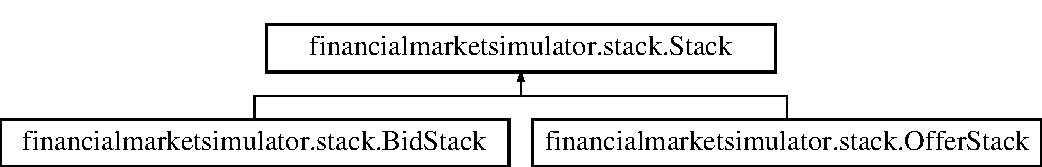
\includegraphics[height=2.000000cm]{classfinancialmarketsimulator_1_1stack_1_1_stack}
\end{center}
\end{figure}
\subsection*{Public Member Functions}
\begin{DoxyCompactItemize}
\item 
void \hyperlink{classfinancialmarketsimulator_1_1stack_1_1_stack_a923eeb3696e2bbb208516defd3039213}{push} (\hyperlink{classfinancialmarketsimulator_1_1stack_1_1_market_entry_attempt_node}{Market\+Entry\+Attempt\+Node} node)  throws Interrupted\+Exception 
\item 
\hyperlink{classfinancialmarketsimulator_1_1stack_1_1_market_entry_attempt_node}{Market\+Entry\+Attempt\+Node} \hyperlink{classfinancialmarketsimulator_1_1stack_1_1_stack_acf0de0447fa83242a8409bc5903ca215}{pop} ()  throws Empty\+Exception, Interrupted\+Exception 
\end{DoxyCompactItemize}
\subsection*{Protected Member Functions}
\begin{DoxyCompactItemize}
\item 
boolean \hyperlink{classfinancialmarketsimulator_1_1stack_1_1_stack_a2566c4821f0d3091cdac87b5ee7404bf}{try\+Push} (\hyperlink{classfinancialmarketsimulator_1_1stack_1_1_market_entry_attempt_node}{Market\+Entry\+Attempt\+Node} node)
\item 
\hyperlink{classfinancialmarketsimulator_1_1stack_1_1_market_entry_attempt_node}{Market\+Entry\+Attempt\+Node} \hyperlink{classfinancialmarketsimulator_1_1stack_1_1_stack_aacd57a41238742e12b8ee9f20b93b162}{try\+Pop} ()  throws Empty\+Exception 
\end{DoxyCompactItemize}


\subsection{Detailed Description}
\begin{DoxyAuthor}{Author}
Madimetja 
\end{DoxyAuthor}


Definition at line 14 of file Stack.\+java.



\subsection{Member Function Documentation}
\hypertarget{classfinancialmarketsimulator_1_1stack_1_1_stack_acf0de0447fa83242a8409bc5903ca215}{\index{financialmarketsimulator\+::stack\+::\+Stack@{financialmarketsimulator\+::stack\+::\+Stack}!pop@{pop}}
\index{pop@{pop}!financialmarketsimulator\+::stack\+::\+Stack@{financialmarketsimulator\+::stack\+::\+Stack}}
\subsubsection[{pop}]{\setlength{\rightskip}{0pt plus 5cm}{\bf Market\+Entry\+Attempt\+Node} financialmarketsimulator.\+stack.\+Stack.\+pop (
\begin{DoxyParamCaption}
{}
\end{DoxyParamCaption}
) throws {\bf Empty\+Exception}, Interrupted\+Exception}}\label{classfinancialmarketsimulator_1_1stack_1_1_stack_acf0de0447fa83242a8409bc5903ca215}


Definition at line 51 of file Stack.\+java.

\hypertarget{classfinancialmarketsimulator_1_1stack_1_1_stack_a923eeb3696e2bbb208516defd3039213}{\index{financialmarketsimulator\+::stack\+::\+Stack@{financialmarketsimulator\+::stack\+::\+Stack}!push@{push}}
\index{push@{push}!financialmarketsimulator\+::stack\+::\+Stack@{financialmarketsimulator\+::stack\+::\+Stack}}
\subsubsection[{push}]{\setlength{\rightskip}{0pt plus 5cm}void financialmarketsimulator.\+stack.\+Stack.\+push (
\begin{DoxyParamCaption}
\item[{{\bf Market\+Entry\+Attempt\+Node}}]{node}
\end{DoxyParamCaption}
) throws Interrupted\+Exception}}\label{classfinancialmarketsimulator_1_1stack_1_1_stack_a923eeb3696e2bbb208516defd3039213}


Definition at line 27 of file Stack.\+java.

\hypertarget{classfinancialmarketsimulator_1_1stack_1_1_stack_aacd57a41238742e12b8ee9f20b93b162}{\index{financialmarketsimulator\+::stack\+::\+Stack@{financialmarketsimulator\+::stack\+::\+Stack}!try\+Pop@{try\+Pop}}
\index{try\+Pop@{try\+Pop}!financialmarketsimulator\+::stack\+::\+Stack@{financialmarketsimulator\+::stack\+::\+Stack}}
\subsubsection[{try\+Pop}]{\setlength{\rightskip}{0pt plus 5cm}{\bf Market\+Entry\+Attempt\+Node} financialmarketsimulator.\+stack.\+Stack.\+try\+Pop (
\begin{DoxyParamCaption}
{}
\end{DoxyParamCaption}
) throws {\bf Empty\+Exception}\hspace{0.3cm}{\ttfamily [protected]}}}\label{classfinancialmarketsimulator_1_1stack_1_1_stack_aacd57a41238742e12b8ee9f20b93b162}


Definition at line 37 of file Stack.\+java.

\hypertarget{classfinancialmarketsimulator_1_1stack_1_1_stack_a2566c4821f0d3091cdac87b5ee7404bf}{\index{financialmarketsimulator\+::stack\+::\+Stack@{financialmarketsimulator\+::stack\+::\+Stack}!try\+Push@{try\+Push}}
\index{try\+Push@{try\+Push}!financialmarketsimulator\+::stack\+::\+Stack@{financialmarketsimulator\+::stack\+::\+Stack}}
\subsubsection[{try\+Push}]{\setlength{\rightskip}{0pt plus 5cm}boolean financialmarketsimulator.\+stack.\+Stack.\+try\+Push (
\begin{DoxyParamCaption}
\item[{{\bf Market\+Entry\+Attempt\+Node}}]{node}
\end{DoxyParamCaption}
)\hspace{0.3cm}{\ttfamily [protected]}}}\label{classfinancialmarketsimulator_1_1stack_1_1_stack_a2566c4821f0d3091cdac87b5ee7404bf}


Definition at line 21 of file Stack.\+java.



The documentation for this class was generated from the following file\+:\begin{DoxyCompactItemize}
\item 
C\+:/\+Users/\+Madimetja/\+Documents/\+Git\+Hub/bravo/\+Financial\+Market\+Simulator/src/financialmarketsimulator/stack/\hyperlink{_stack_8java}{Stack.\+java}\end{DoxyCompactItemize}

\hypertarget{classstack_package_unit_tests_1_1_stack_unit_test}{\section{stack\+Package\+Unit\+Tests.\+Stack\+Unit\+Test Class Reference}
\label{classstack_package_unit_tests_1_1_stack_unit_test}\index{stack\+Package\+Unit\+Tests.\+Stack\+Unit\+Test@{stack\+Package\+Unit\+Tests.\+Stack\+Unit\+Test}}
}
\subsection*{Public Member Functions}
\begin{DoxyCompactItemize}
\item 
\hypertarget{classstack_package_unit_tests_1_1_stack_unit_test_a21d7f0fe59add6adeba3968a0efd6665}{void {\bfseries set\+Up} ()}\label{classstack_package_unit_tests_1_1_stack_unit_test_a21d7f0fe59add6adeba3968a0efd6665}

\item 
\hypertarget{classstack_package_unit_tests_1_1_stack_unit_test_a2e35176b63667c6e025495e811b5d473}{void {\bfseries tear\+Down} ()}\label{classstack_package_unit_tests_1_1_stack_unit_test_a2e35176b63667c6e025495e811b5d473}

\end{DoxyCompactItemize}
\subsection*{Static Public Member Functions}
\begin{DoxyCompactItemize}
\item 
\hypertarget{classstack_package_unit_tests_1_1_stack_unit_test_ab44e5f0e6f4dfcdc89b416109dd7db11}{static void {\bfseries set\+Up\+Class} ()}\label{classstack_package_unit_tests_1_1_stack_unit_test_ab44e5f0e6f4dfcdc89b416109dd7db11}

\item 
\hypertarget{classstack_package_unit_tests_1_1_stack_unit_test_ab065aabd4484126579c30a5ab4acb941}{static void {\bfseries tear\+Down\+Class} ()}\label{classstack_package_unit_tests_1_1_stack_unit_test_ab065aabd4484126579c30a5ab4acb941}

\end{DoxyCompactItemize}


\subsection{Detailed Description}
\begin{DoxyAuthor}{Author}
Madimetja 
\end{DoxyAuthor}


Definition at line 20 of file Stack\+Unit\+Test.\+java.



The documentation for this class was generated from the following file\+:\begin{DoxyCompactItemize}
\item 
C\+:/\+Users/\+Madimetja/\+Documents/\+Git\+Hub/bravo/\+Financial\+Market\+Simulator/test/stack\+Package\+Unit\+Tests/Stack\+Unit\+Test.\+java\end{DoxyCompactItemize}

\hypertarget{interfacefinancialmarketsimulator_1_1_trade}{\section{financialmarketsimulator.\+Trade Interface Reference}
\label{interfacefinancialmarketsimulator_1_1_trade}\index{financialmarketsimulator.\+Trade@{financialmarketsimulator.\+Trade}}
}
Inheritance diagram for financialmarketsimulator.\+Trade\+:\begin{figure}[H]
\begin{center}
\leavevmode
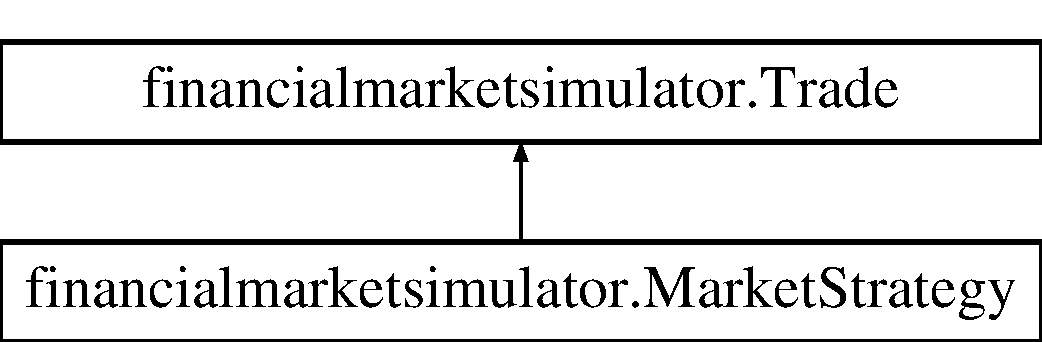
\includegraphics[height=2.000000cm]{interfacefinancialmarketsimulator_1_1_trade}
\end{center}
\end{figure}
\subsection*{Public Member Functions}
\begin{DoxyCompactItemize}
\item 
\hypertarget{interfacefinancialmarketsimulator_1_1_trade_aba2e7742e3c7a477417abb741eb049af}{\hyperlink{classfinancialmarketsimulator_1_1_market_entry_attempt}{Market\+Entry\+Attempt} {\bfseries make\+Offer} ()}\label{interfacefinancialmarketsimulator_1_1_trade_aba2e7742e3c7a477417abb741eb049af}

\item 
\hypertarget{interfacefinancialmarketsimulator_1_1_trade_ab84e578afb7f519b018ebc0ffaab4d2a}{\hyperlink{classfinancialmarketsimulator_1_1_market_entry_attempt}{Market\+Entry\+Attempt} {\bfseries make\+Bid} ()}\label{interfacefinancialmarketsimulator_1_1_trade_ab84e578afb7f519b018ebc0ffaab4d2a}

\item 
\hypertarget{interfacefinancialmarketsimulator_1_1_trade_a22d67d3c44faaf8fca8a4fd2d78a3e75}{void {\bfseries retract\+Bid} ()}\label{interfacefinancialmarketsimulator_1_1_trade_a22d67d3c44faaf8fca8a4fd2d78a3e75}

\item 
\hypertarget{interfacefinancialmarketsimulator_1_1_trade_a1a1cbe142a99ac5e08872efea02239f7}{void {\bfseries retract\+Offer} ()}\label{interfacefinancialmarketsimulator_1_1_trade_a1a1cbe142a99ac5e08872efea02239f7}

\item 
\hypertarget{interfacefinancialmarketsimulator_1_1_trade_aa3cfc0cff8e9a08e48cfd70ae870cb8b}{void {\bfseries set\+Strategy} (String strategy)}\label{interfacefinancialmarketsimulator_1_1_trade_aa3cfc0cff8e9a08e48cfd70ae870cb8b}

\item 
\hypertarget{interfacefinancialmarketsimulator_1_1_trade_a2635502a77913bfa79d6a953ee7c3c1f}{\hyperlink{classfinancialmarketsimulator_1_1_market_entry_attempt}{Market\+Entry\+Attempt} {\bfseries search\+Market\+Entry\+Attempt} (\hyperlink{classfinancialmarketsimulator_1_1_market_entry_attempt}{Market\+Entry\+Attempt} entry)}\label{interfacefinancialmarketsimulator_1_1_trade_a2635502a77913bfa79d6a953ee7c3c1f}

\end{DoxyCompactItemize}


\subsection{Detailed Description}
\begin{DoxyAuthor}{Author}
Madimetja 
\end{DoxyAuthor}


Definition at line 12 of file Trade.\+java.



The documentation for this interface was generated from the following file\+:\begin{DoxyCompactItemize}
\item 
C\+:/\+Users/\+Madimetja/\+Documents/\+Git\+Hub/bravo/\+Financial\+Market\+Simulator/src/financialmarketsimulator/Trade.\+java\end{DoxyCompactItemize}

\hypertarget{classfinancialmarketsimulator_1_1receipts_1_1_trade_receipt}{\section{financialmarketsimulator.\+receipts.\+Trade\+Receipt Class Reference}
\label{classfinancialmarketsimulator_1_1receipts_1_1_trade_receipt}\index{financialmarketsimulator.\+receipts.\+Trade\+Receipt@{financialmarketsimulator.\+receipts.\+Trade\+Receipt}}
}
Inheritance diagram for financialmarketsimulator.\+receipts.\+Trade\+Receipt\+:\begin{figure}[H]
\begin{center}
\leavevmode
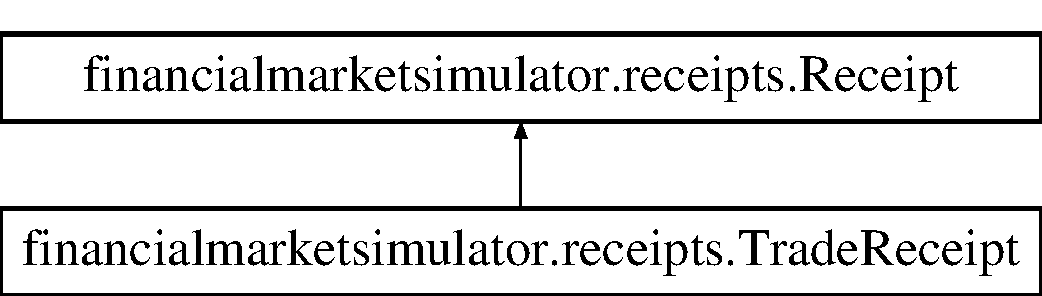
\includegraphics[height=2.000000cm]{classfinancialmarketsimulator_1_1receipts_1_1_trade_receipt}
\end{center}
\end{figure}


\subsection{Detailed Description}
\begin{DoxyAuthor}{Author}
Moeletji 
\end{DoxyAuthor}


Definition at line 13 of file Trade\+Receipt.\+java.



The documentation for this class was generated from the following file\+:\begin{DoxyCompactItemize}
\item 
C\+:/\+Users/\+Madimetja/\+Documents/\+Git\+Hub/bravo/\+Financial\+Market\+Simulator/src/financialmarketsimulator/receipts/\hyperlink{_trade_receipt_8java}{Trade\+Receipt.\+java}\end{DoxyCompactItemize}

\hypertarget{class_trade_unit_test}{\section{Trade\+Unit\+Test Class Reference}
\label{class_trade_unit_test}\index{Trade\+Unit\+Test@{Trade\+Unit\+Test}}
}
\subsection*{Public Member Functions}
\begin{DoxyCompactItemize}
\item 
\hypertarget{class_trade_unit_test_aef602b2b9e5555fc5da1bb749b611ccd}{void {\bfseries set\+Up} ()}\label{class_trade_unit_test_aef602b2b9e5555fc5da1bb749b611ccd}

\item 
\hypertarget{class_trade_unit_test_a34ba2c94e327c25a445241730d3953ef}{void {\bfseries tear\+Down} ()}\label{class_trade_unit_test_a34ba2c94e327c25a445241730d3953ef}

\end{DoxyCompactItemize}
\subsection*{Static Public Member Functions}
\begin{DoxyCompactItemize}
\item 
\hypertarget{class_trade_unit_test_a5be15b13c335f6325b1ee14ef9062a92}{static void {\bfseries set\+Up\+Class} ()}\label{class_trade_unit_test_a5be15b13c335f6325b1ee14ef9062a92}

\item 
\hypertarget{class_trade_unit_test_a12cc028ac0612978efa5400afd4baaa5}{static void {\bfseries tear\+Down\+Class} ()}\label{class_trade_unit_test_a12cc028ac0612978efa5400afd4baaa5}

\end{DoxyCompactItemize}


\subsection{Detailed Description}
\begin{DoxyAuthor}{Author}
Madimetja 
\end{DoxyAuthor}


Definition at line 18 of file Trade\+Unit\+Test.\+java.



The documentation for this class was generated from the following file\+:\begin{DoxyCompactItemize}
\item 
C\+:/\+Users/\+Madimetja/\+Documents/\+Git\+Hub/bravo/\+Financial\+Market\+Simulator/test/Trade\+Unit\+Test.\+java\end{DoxyCompactItemize}

%--- End generated contents ---

% Index
\newpage
\phantomsection
\addcontentsline{toc}{chapter}{Index}
\printindex

\end{document}
